\documentclass{pasa}%

\usepackage{graphicx}
\usepackage{xspace}

\title[PhD thesis summary]{ \bfseries\Large\centering
    \textbf{Ph.D. thesis summary:}\\
    %\vspace{0.1 in}
    A Novel Multidimensional Search for\\ 
    Diboson Resonances in the Boosted Dijet Final State\\
    %\vspace{0.2 in}
    and\\
    %\vspace{0.2 in}
    Encoding Jet Substructure with a Deep Neural Network\\
}

%% Please note that the command \and is not supported in \author.
\author[Thea Klaeboe Aarrestad]{Thea Klaeboe Aarrestad
\affil{University of Zurich}
}


\jid{}
\doi{10.1103/PhysRevD.97.072006; 10.1007/JHEP03(2017)162; cds.cern.ch/record/2256875 (CERN public document); cds.cern.ch/record/2668755 (submitted to EPJC) }


\usepackage{aas_macros}
\usepackage{hyperref} 
\hypersetup{colorlinks,citecolor=black,linkcolor=black,urlcolor=black}
%\usepackage{lineno}
%\linenumbers
%%%%%%%%%%%%%%%%%%%%%%%%%%%%%%%%%%%%%%%%%%%%%%%%%%%%%%%%%%%%%%%%%%%%
%
%  Common definitions
%
%  N.B. use of \providecommand rather than \newcommand means
%       that a definition is ignored if already specified
%
%                                              L. Taylor 18 Feb 2005
%%%%%%%%%%%%%%%%%%%%%%%%%%%%%%%%%%%%%%%%%%%%%%%%%%%%%%%%%%%%%%%%%%%%
% PRIVATE
\newcommand{\mVV}{\ensuremath{m_{\VV}}\xspace}
\newcommand{\mqV}{\ensuremath{m_{\qo\PV}}\xspace}
\newcommand{\mjj}{\ensuremath{m_\mathrm{jj}}}
\newcommand{\mJ}{\ensuremath{m_{\text{jet}}}}
\newcommand{\nsubj}{\ensuremath{\tau_{21}}}
\newcommand{\ddt}{\ensuremath{\tau_{21}^{DDT}}}
\newcommand{\ktilde}{\ensuremath{\tilde{k}}}
\newcommand{\VV}{\ensuremath{\PV\PV}\xspace}
\newcommand{\WW}{\ensuremath{\PW\PW}\xspace}
\newcommand{\WZ}{\ensuremath{\PW\PZ}\xspace}
\newcommand{\ZZ}{\ensuremath{\PZ\PZ}\xspace}
\newcommand{\mX}{\ensuremath{\text{M}_{\text{X}}}}%
% Some shorthand
% turn off italics
\newcommand {\etal}{\mbox{et al.}\xspace} %et al. - no preceding comma
\newcommand {\ie}{\mbox{i.e.}\xspace}     %i.e.
\newcommand {\eg}{\mbox{e.g.}\xspace}     %e.g.
\newcommand {\etc}{\mbox{etc.}\xspace}     %etc.
\newcommand {\vs}{\mbox{\sl vs.}\xspace}      %vs.
\newcommand {\mdash}{\ensuremath{\mathrm{-}}} % for use within formulas

% some terms whose definition we may change
\newcommand {\Lone}{Level-1\xspace} % Level-1 or L1 ?
\newcommand {\Ltwo}{Level-2\xspace}
\newcommand {\Lthree}{Level-3\xspace}

% Some software programs (alphabetized)
\providecommand{\ACERMC} {\textsc{AcerMC}\xspace}
\newcommand{\amcatnlo}{\textsc{madgraph5\_amc@nlo}\xspace}
\providecommand{\ALPGEN} {{\textsc{alpgen}}\xspace}
\providecommand{\CHARYBDIS} {{\textsc{charybdis}}\xspace}
\providecommand{\CMKIN} {\textsc{cmkin}\xspace}
\providecommand{\CMSIM} {{\textsc{cmsim}}\xspace}
\providecommand{\CMSSW} {{\textsc{cmssw}}\xspace}
\providecommand{\COBRA} {{\textsc{cobra}}\xspace}
\providecommand{\COCOA} {{\textsc{cocoa}}\xspace}
\providecommand{\COMPHEP} {\textsc{CompHEP}\xspace}
\providecommand{\EVTGEN} {{\textsc{evtgen}}\xspace}
\providecommand{\FAMOS} {{\textsc{famos}}\xspace}
\providecommand{\GARCON} {\textsc{garcon}\xspace}
\providecommand{\GARFIELD} {{\textsc{garfield}}\xspace}
\providecommand{\GEANE} {{\textsc{geane}}\xspace}
\providecommand{\GEANTfour} {{\textsc{geant4}}\xspace}
\providecommand{\GEANTthree} {{\textsc{geant3}}\xspace}
\providecommand{\GEANT} {{\textsc{geant}}\xspace}
\providecommand{\HDECAY} {\textsc{hdecay}\xspace}
\providecommand{\HERWIG} {{\textsc{herwig}}\xspace}
\providecommand{\HIGLU} {{\textsc{higlu}}\xspace}
\providecommand{\HIJING} {{\textsc{hijing}}\xspace}
\providecommand{\IGUANA} {\textsc{iguana}\xspace}
\providecommand{\ISAJET} {{\textsc{isajet}}\xspace}
\providecommand{\ISAPYTHIA} {{\textsc{isapythia}}\xspace}
\providecommand{\ISASUGRA} {{\textsc{isasugra}}\xspace}
\providecommand{\ISASUSY} {{\textsc{isasusy}}\xspace}
\providecommand{\ISAWIG} {{\textsc{isawig}}\xspace}
\providecommand{\MADGRAPH} {\textsc{MadGraph}\xspace}
\providecommand{\MCATNLO} {\textsc{mc@nlo}\xspace}
\providecommand{\MCFM} {\textsc{mcfm}\xspace}
\providecommand{\MILLEPEDE} {{\textsc{millepede}}\xspace}
\providecommand{\ORCA} {{\textsc{orca}}\xspace}
\providecommand{\OSCAR} {{\textsc{oscar}}\xspace}
\providecommand{\PHOTOS} {\textsc{photos}\xspace}
\providecommand{\POWHEG} {{\textsc{powheg}}\xspace}
\providecommand{\PROSPINO} {\textsc{prospino}\xspace}
\providecommand{\PYTHIA} {{\textsc{pythia}}\xspace}
\providecommand{\SHERPA} {{\textsc{sherpa}}\xspace}
\providecommand{\TAUOLA} {\textsc{tauola}\xspace}
\providecommand{\TOPREX} {\textsc{TopReX}\xspace}
\providecommand{\XDAQ} {{\textsc{xdaq}}\xspace}

%%%%%%%%%% Experiments %%%%%%%%%%%%%%%%%%

\newcommand {\DZERO}{D\O\xspace}     %etc.

%%%%%%%%%% Measurements and units %%%%%%%%%%%%%%%%%%

\newcommand{\de}{\ensuremath{^\circ}\xspace}
\newcommand{\ten}[1]{\ensuremath{\times \text{10}^\text{#1}}}
\newcommand{\unit}[1]{\ensuremath{\text{\,#1}}\xspace}
\newcommand{\mum}{\ensuremath{\,\mu\text{m}}\xspace}
\newcommand{\micron}{\ensuremath{\,\mu\text{m}}\xspace}
\newcommand{\cm}{\ensuremath{\,\text{cm}}\xspace}
\newcommand{\mm}{\ensuremath{\,\text{mm}}\xspace}
\newcommand{\mus}{\ensuremath{\,\mu\text{s}}\xspace}
\newcommand{\keV}{\ensuremath{\,\text{ke\hspace{-.08em}V}}\xspace}
\newcommand{\MeV}{\ensuremath{\,\text{Me\hspace{-.08em}V}}\xspace}
\newcommand{\GeV}{\ensuremath{\,\text{Ge\hspace{-.08em}V}}\xspace}
\newcommand{\TeV}{\ensuremath{\,\text{Te\hspace{-.08em}V}}\xspace}
\newcommand{\PeV}{\ensuremath{\,\text{Pe\hspace{-.08em}V}}\xspace}
\newcommand{\keVc}{\ensuremath{{\,\text{ke\hspace{-.08em}V\hspace{-0.16em}/\hspace{-0.08em}}c}}\xspace}
\newcommand{\MeVc}{\ensuremath{{\,\text{Me\hspace{-.08em}V\hspace{-0.16em}/\hspace{-0.08em}}c}}\xspace}
\newcommand{\GeVc}{\ensuremath{{\,\text{Ge\hspace{-.08em}V\hspace{-0.16em}/\hspace{-0.08em}}c}}\xspace}
\newcommand{\TeVc}{\ensuremath{{\,\text{Te\hspace{-.08em}V\hspace{-0.16em}/\hspace{-0.08em}}c}}\xspace}
\newcommand{\keVcc}{\ensuremath{{\,\text{ke\hspace{-.08em}V\hspace{-0.16em}/\hspace{-0.08em}}c^\text{2}}}\xspace}
\newcommand{\MeVcc}{\ensuremath{{\,\text{Me\hspace{-.08em}V\hspace{-0.16em}/\hspace{-0.08em}}c^\text{2}}}\xspace}
\newcommand{\GeVcc}{\ensuremath{{\,\text{Ge\hspace{-.08em}V\hspace{-0.16em}/\hspace{-0.08em}}c^\text{2}}}\xspace}
\newcommand{\TeVcc}{\ensuremath{{\,\text{Te\hspace{-.08em}V\hspace{-0.16em}/\hspace{-0.08em}}c^\text{2}}}\xspace}
\newcommand{\MPl}{\ensuremath{M_\mathrm{Pl}}\xspace}
\newcommand{\bMPl}{\ensuremath{\overline{M}_\mathrm{Pl}}\xspace}

\newcommand{\pbinv} {\mbox{\ensuremath{\,\text{pb}^\text{$-$1}}}\xspace}
\newcommand{\fbinv} {\mbox{\ensuremath{\,\text{fb}^\text{$-$1}}}\xspace}
\newcommand{\nbinv} {\mbox{\ensuremath{\,\text{nb}^\text{$-$1}}}\xspace}
\newcommand{\percms}{\ensuremath{\,\text{cm}^\text{$-$2}\,\text{s}^\text{$-$1}}\xspace}
\newcommand{\lumi}{\ensuremath{\mathcal{L}}\xspace}
\newcommand{\Lumi}{\ensuremath{\mathcal{L}}\xspace}%both upper and lower
%
% Need a convention here:
\newcommand{\LvLow}  {\ensuremath{\mathcal{L}=\text{10}^\text{32}\,\text{cm}^\text{$-$2}\,\text{s}^\text{$-$1}}\xspace}
\newcommand{\LLow}   {\ensuremath{\mathcal{L}=\text{10}^\text{33}\,\text{cm}^\text{$-$2}\,\text{s}^\text{$-$1}}\xspace}
\newcommand{\lowlumi}{\ensuremath{\mathcal{L}=\text{2}\times \text{10}^\text{33}\,\text{cm}^\text{$-$2}\,\text{s}^\text{$-$1}}\xspace}
\newcommand{\LMed}   {\ensuremath{\mathcal{L}=\text{2}\times \text{10}^\text{33}\,\text{cm}^\text{$-$2}\,\text{s}^\text{$-$1}}\xspace}
\newcommand{\LHigh}  {\ensuremath{\mathcal{L}=\text{10}^\text{34}\,\text{cm}^\text{$-$2}\,\text{s}^\text{$-$1}}\xspace}
\newcommand{\hilumi} {\ensuremath{\mathcal{L}=\text{10}^\text{34}\,\text{cm}^\text{$-$2}\,\text{s}^\text{$-$1}}\xspace}


%%%%%%%%%% Some usual physics terms/symbols %%%%%%%%%%%%%%%%%%

\newcommand{\kt}{\ensuremath{k_{\mathrm{T}}}\xspace}
\newcommand{\wangle}{\ensuremath{\sin^{2}\theta_{\text{eff}}^\text{lept}(M^2_\mathrm{Z})}\xspace}
\newcommand{\stat}{\ensuremath{\,\text{(stat.)}}\xspace}
\newcommand{\syst}{\ensuremath{\,\text{(syst.)}}\xspace}
\newcommand{\AFB}{\ensuremath{A_\text{FB}}\xspace}
\newcommand{\MD}{\ensuremath{{M_\mathrm{D}}}\xspace}% ED mass
\newcommand{\Mpl}{\ensuremath{{M_\mathrm{Pl}}}\xspace}% Planck mass
\newcommand{\Rinv} {\ensuremath{{R}^{-1}}\xspace}

\providecommand{\Em}{\ensuremath{E\hspace{-0.6em}/}\xspace}
\providecommand{\Pm}{\ensuremath{p\hspace{-0.5em}/}\xspace}
\providecommand{\PTm}{\ensuremath{{p}_\mathrm{T}\hspace{-1.02em}/}\xspace}
\newcommand{\PT}{\ensuremath{p_{\mathrm{T}}}\xspace}
\newcommand{\pt}{\ensuremath{p_{\mathrm{T}}}\xspace}
\newcommand{\Vpt}{\ensuremath{{\vec p}_{\mathrm{T}}}\xspace}
\newcommand{\ET}{\ensuremath{E_{\mathrm{T}}}\xspace}
\newcommand{\et}{\ensuremath{E_{\mathrm{T}}}\xspace}
\newcommand{\HT}{\ensuremath{H_{\mathrm{T}}}\xspace}
\newcommand{\Etmiss}{\ensuremath{E_{\mathrm{T}\!{\rm miss}}}}
\newcommand{\ETm}{\ensuremath{E_{\mathrm{T}}^{\text{miss}}}\xspace}
\newcommand{\MET}{\ensuremath{E_{\mathrm{T}}^{\text{miss}}}\xspace}
\newcommand{\ETmiss}{\ensuremath{E_{\mathrm{T}}^{\text{miss}}}\xspace}
\newcommand{\VEtmiss}{\ensuremath{{\vec E}_{\mathrm{T}}^{\;\text{miss}}}\xspace}
\newcommand{\ptvecmiss}{\ensuremath{{\vec p}_{\mathrm{T}}^{\kern1pt\text{miss}}}\xspace}
\providecommand{\PTslash}{\ensuremath{{p}_\mathrm{T}\hspace{-1.02em}/}\xspace}
\providecommand{\ETslash}{\ensuremath{E_{\mathrm{T}}\hspace{-1.1em}/}\xspace}

%%%%%%%%%% SM particles %%%%%%%%%%%%%%%%%%

\newcommand{\BC}{\ensuremath{{B_{\mathrm{c}}}}\xspace}
\newcommand{\JPsi}{\ensuremath{{J}\hspace{-.08em}/\hspace{-.14em}\psi}\xspace}
\providecommand{\cPJgy}{\JPsi} % J/Psi (no mass)
\newcommand{\bspsiphi}{\ensuremath{B_s \to \JPsi\, \phi}\xspace}
\providecommand{\JPsi}{\ensuremath{\mathrm{J}\hspace{-.08em}/\hspace{-.14em}\psi}\xspace}

%quarks
\newcommand{\cPg}{\ensuremath{\mathrm{g}}} % generic gluon
\newcommand{\cPq}{\ensuremath{\mathrm{q}}}
\newcommand{\cPaq}{\ensuremath{\overline{\mathrm{q}}}}
\newcommand{\qqbarpr}{\ensuremath{\cPq\cPaq^({}'^){}}\xspace}
\newcommand{\qqbar}{\ensuremath{\cPq\cPaq}\xspace}
\newcommand{\cPqt}{\ensuremath{\mathrm{t}}} % t for t quark
\newcommand{\cPqb}{\ensuremath{\mathrm{b}}} % b for b quark
\newcommand{\bbarc}{\ensuremath{{\overline{b}c}}\xspace}
\newcommand{\bbbar}{\ensuremath{{\mathrm{b}\overline{\mathrm{b}}}}\xspace}
\newcommand{\ccbar}{\ensuremath{{c\overline{c}}}\xspace}
\providecommand{\ttbar}{\ensuremath{\mathrm{t}\overline{\mathrm{t}}}\xspace}

%leptons/neutrinos
\newcommand{\Pgn}{\ensuremath{\nu}}%neutrino
\providecommand{\cPgn}{\ensuremath{\nu}\xspace} % generic neutrino
\newcommand{\EE}{\ensuremath{e^+e^-}\xspace}
\newcommand{\MM}{\ensuremath{\mu^+\mu^-}\xspace}
\newcommand{\TT}{\ensuremath{\tau^+\tau^-}\xspace}

%bosons
\providecommand{\PZ}{\ensuremath{\mathrm{Z}}\xspace}
\providecommand{\cPZ}{\Z} % plain Z (no superscript 0)
\providecommand{\PW}{\ensuremath{\mathrm{W}}\xspace}
\providecommand{\PV}{\ensuremath{\mathrm{V}}\xspace}
\providecommand{\PH}{\ensuremath{\mathrm{H}}\xspace}
\providecommand{\PWL}{\ensuremath{\mathrm{W}_{\mathrm{L}}}\xspace}
\providecommand{\PWT}{\ensuremath{\mathrm{W}_{\mathrm{T}}}\xspace}

%%%%%%%%%% BSM particles %%%%%%%%%%%%%%%%%%

\providecommand{\Zpr}{\ensuremath{\mathrm{Z}^\prime}\xspace}
\providecommand{\cPZpr}{\Zpr} % plain Z'
\providecommand{\PZpr}{\ensuremath{\mathrm{Z}^\prime}\xspace} % plain Z' using prime
\providecommand{\Wpr}{\ensuremath{\mathrm{W}^\prime}\xspace}
\providecommand{\cPWpr}{\Wpr} % plain W'
\providecommand{\PWpr}{\ensuremath{\mathrm{W}^\prime}\xspace} % plain W' using prime
\providecommand{\PVpr}{\ensuremath{\mathrm{V}^\prime}\xspace} % plain V' using prime
\providecommand{\BulkG}{\ensuremath{\mathrm{G}_\mathrm{bulk}}\xspace}

%%%%%%%%%%%%%  E-gamma definitions %%%%%%%%%%%%%%
\newcommand{\HGG}{\ensuremath{\mathrm{H}\to\gamma\gamma}}
\newcommand{\gev}{\GeV}
\newcommand{\GAMJET}{\ensuremath{\gamma + \text{jet}}}
\newcommand{\PPTOJETS}{\ensuremath{\mathrm{pp}\to\text{jets}}}
\newcommand{\PPTOGG}{\ensuremath{\mathrm{pp}\to\gamma\gamma}}
\newcommand{\PPTOGAMJET}{\ensuremath{\mathrm{pp}\to\gamma + \mathrm{jet}}}
\newcommand{\MH}{\ensuremath{\mathrm{M_{\mathrm{H}}}}}
\newcommand{\RNINE}{\ensuremath{\mathrm{R}_\mathrm{9}}}
\newcommand{\DR}{\ensuremath{\Delta\mathrm{R}}}

%%%%%%%%%%%%%%% other stuff %%%%%%%%%%%%
\providecommand{\dd}[2]{\ensuremath{\frac{\mathrm{d} #1}{\mathrm{d} #2}}}

\newcommand{\ga}{\ensuremath{\gtrsim}}
\newcommand{\la}{\ensuremath{\lesssim}}
\newcommand{\swsq}{\ensuremath{\sin^2\theta_W}\xspace}
\newcommand{\cwsq}{\ensuremath{\cos^2\theta_W}\xspace}
\newcommand{\tanb}{\ensuremath{\tan\beta}\xspace}
\newcommand{\tanbsq}{\ensuremath{\tan^{2}\beta}\xspace}
\newcommand{\sidb}{\ensuremath{\sin 2\beta}\xspace}
\newcommand{\alpS}{\ensuremath{\alpha_S}\xspace}
\newcommand{\alpt}{\ensuremath{\tilde{\alpha}}\xspace}

\newcommand{\QL}{\ensuremath{Q_L}\xspace}
\newcommand{\sQ}{\ensuremath{\tilde{Q}}\xspace}
\newcommand{\sQL}{\ensuremath{\tilde{Q}_L}\xspace}
\newcommand{\ULC}{\ensuremath{U_L^C}\xspace}
\newcommand{\sUC}{\ensuremath{\tilde{U}^C}\xspace}
\newcommand{\sULC}{\ensuremath{\tilde{U}_L^C}\xspace}
\newcommand{\DLC}{\ensuremath{D_L^C}\xspace}
\newcommand{\sDC}{\ensuremath{\tilde{D}^C}\xspace}
\newcommand{\sDLC}{\ensuremath{\tilde{D}_L^C}\xspace}
\newcommand{\LL}{\ensuremath{L_L}\xspace}
\newcommand{\sL}{\ensuremath{\tilde{L}}\xspace}
\newcommand{\sLL}{\ensuremath{\tilde{L}_L}\xspace}
\newcommand{\ELC}{\ensuremath{E_L^C}\xspace}
\newcommand{\sEC}{\ensuremath{\tilde{E}^C}\xspace}
\newcommand{\sELC}{\ensuremath{\tilde{E}_L^C}\xspace}
\newcommand{\sEL}{\ensuremath{\tilde{E}_L}\xspace}
\newcommand{\sER}{\ensuremath{\tilde{E}_R}\xspace}
\newcommand{\sFer}{\ensuremath{\tilde{f}}\xspace}
\newcommand{\sQua}{\ensuremath{\tilde{q}}\xspace}
\newcommand{\sUp}{\ensuremath{\tilde{u}}\xspace}
\newcommand{\suL}{\ensuremath{\tilde{u}_L}\xspace}
\newcommand{\suR}{\ensuremath{\tilde{u}_R}\xspace}
\newcommand{\sDw}{\ensuremath{\tilde{d}}\xspace}
\newcommand{\sdL}{\ensuremath{\tilde{d}_L}\xspace}
\newcommand{\sdR}{\ensuremath{\tilde{d}_R}\xspace}
\newcommand{\sTop}{\ensuremath{\tilde{t}}\xspace}
\newcommand{\stL}{\ensuremath{\tilde{t}_L}\xspace}
\newcommand{\stR}{\ensuremath{\tilde{t}_R}\xspace}
\newcommand{\stone}{\ensuremath{\tilde{t}_1}\xspace}
\newcommand{\sttwo}{\ensuremath{\tilde{t}_2}\xspace}
\newcommand{\sBot}{\ensuremath{\tilde{b}}\xspace}
\newcommand{\sbL}{\ensuremath{\tilde{b}_L}\xspace}
\newcommand{\sbR}{\ensuremath{\tilde{b}_R}\xspace}
\newcommand{\sbone}{\ensuremath{\tilde{b}_1}\xspace}
\newcommand{\sbtwo}{\ensuremath{\tilde{b}_2}\xspace}
\newcommand{\sLep}{\ensuremath{\tilde{l}}\xspace}
\newcommand{\sLepC}{\ensuremath{\tilde{l}^C}\xspace}
\newcommand{\sEl}{\ensuremath{\tilde{e}}\xspace}
\newcommand{\sElC}{\ensuremath{\tilde{e}^C}\xspace}
\newcommand{\seL}{\ensuremath{\tilde{e}_L}\xspace}
\newcommand{\seR}{\ensuremath{\tilde{e}_R}\xspace}
\newcommand{\snL}{\ensuremath{\tilde{\nu}_L}\xspace}
\newcommand{\sMu}{\ensuremath{\tilde{\mu}}\xspace}
\newcommand{\sNu}{\ensuremath{\tilde{\nu}}\xspace}
\newcommand{\sTau}{\ensuremath{\tilde{\tau}}\xspace}
\newcommand{\Glu}{\ensuremath{g}\xspace}
\newcommand{\sGlu}{\ensuremath{\tilde{g}}\xspace}
\newcommand{\Wpm}{\ensuremath{W^{\pm}}\xspace}
\newcommand{\sWpm}{\ensuremath{\tilde{W}^{\pm}}\xspace}
\newcommand{\Wz}{\ensuremath{W^{0}}\xspace}
\newcommand{\sWz}{\ensuremath{\tilde{W}^{0}}\xspace}
\newcommand{\sWino}{\ensuremath{\tilde{W}}\xspace}
\newcommand{\Bz}{\ensuremath{B^{0}}\xspace}
\newcommand{\sBz}{\ensuremath{\tilde{B}^{0}}\xspace}
\newcommand{\sBino}{\ensuremath{\tilde{B}}\xspace}
\newcommand{\Zz}{\ensuremath{Z^{0}}\xspace}
\newcommand{\sZino}{\ensuremath{\tilde{Z}^{0}}\xspace}
\newcommand{\sGam}{\ensuremath{\tilde{\gamma}}\xspace}
\newcommand{\chiz}{\ensuremath{\tilde{\chi}^{0}}\xspace}
\newcommand{\chip}{\ensuremath{\tilde{\chi}^{+}}\xspace}
\newcommand{\chim}{\ensuremath{\tilde{\chi}^{-}}\xspace}
\newcommand{\chipm}{\ensuremath{\tilde{\chi}^{\pm}}\xspace}
\newcommand{\Hone}{\ensuremath{H_{d}}\xspace}
\newcommand{\sHone}{\ensuremath{\tilde{H}_{d}}\xspace}
\newcommand{\Htwo}{\ensuremath{H_{u}}\xspace}
\newcommand{\sHtwo}{\ensuremath{\tilde{H}_{u}}\xspace}
\newcommand{\sHig}{\ensuremath{\tilde{H}}\xspace}
\newcommand{\sHa}{\ensuremath{\tilde{H}_{a}}\xspace}
\newcommand{\sHb}{\ensuremath{\tilde{H}_{b}}\xspace}
\newcommand{\sHpm}{\ensuremath{\tilde{H}^{\pm}}\xspace}
\newcommand{\hz}{\ensuremath{h^{0}}\xspace}
\newcommand{\Hz}{\ensuremath{H^{0}}\xspace}
\newcommand{\Az}{\ensuremath{A^{0}}\xspace}
\newcommand{\Hpm}{\ensuremath{H^{\pm}}\xspace}
\newcommand{\sGra}{\ensuremath{\tilde{G}}\xspace}
%
\newcommand{\mtil}{\ensuremath{\tilde{m}}\xspace}
%
\newcommand{\rpv}{\ensuremath{\rlap{\kern.2em/}R}\xspace}
\newcommand{\LLE}{\ensuremath{LL\bar{E}}\xspace}
\newcommand{\LQD}{\ensuremath{LQ\bar{D}}\xspace}
\newcommand{\UDD}{\ensuremath{\overline{UDD}}\xspace}
\newcommand{\Lam}{\ensuremath{\lambda}\xspace}
\newcommand{\Lamp}{\ensuremath{\lambda'}\xspace}
\newcommand{\Lampp}{\ensuremath{\lambda''}\xspace}
%
\newcommand{\spinbd}[2]{\ensuremath{\bar{#1}_{\dot{#2}}}\xspace}


%%%%%%%%%%%%%%%%%%%%%%%%%%%%%%%%%%%%%%%%%%%%%%%%%%%%%%%%%%%%%%%%%%%%
%
% Hyphenations (only need to add here if you get a nasty word break)
%
\hyphenation{en-viron-men-tal}%    just an example

\begin{document}

\begin{frontmatter}
\maketitle
\begin{abstract}
In this thesis I seek answers to some of the most fundamental open questions in particle physics: why is the Higgs boson mass we measured at 125 GeV so much lighter than what we would have predicted when taking into account loop corrections from energy scales up to the Planck scale? And why is gravity so weak compared to the other known forces arising from electroweak and QCD interactions? These are both aspects of the same problem, referred to as the "hierarchy problem". I look for solutions to these questions in the form of extensions of the Standard Model of particle physics, by comparing the physics of high-energy collisions with such alternate models. Specifically, I look for new particles predicted by Composite Higgs models, offering an answer to the first question, and warped extra dimensions theories, attempting to explain both the former and the latter. This thesis presents three different searches for new heavy resonances that decay to a pair of vector bosons in the all-hadronic final state with the CMS detector at the Large Hadron Collider (LHC). The diboson final states under consideration are challenging to resolve due to the bosons being highly energetic (“boosted”), resulting in the two quarks from the decay being collimated and merging into a single jet. This leads to a dijet final state topology where each jet displays substructure in its spatial distribution of energy. I present the results of three different searches I have done, with a number of improvements in techniques that have benefited my analyses, as well as dozens of other measurements done at CMS, ending with the development of a novel multi-dimensional search method yielding a significant improvement in analysis sensitivity and introducing a new way of doing model-independent searches at LHC. 

% The first search I will present was one of the two first CMS searches in boosted final states with 13 TeV data to become published, and the first to take advantage of jet substructure at the trigger level. It was a high-profile analysis due to an observed excess at 8 TeV, and I brought it to a published result within 5 months of first collisions with a center of mass of 13 TeV.. For the second search, I optimized and commissioned a new pileup-resistant, perturbatively robust, vector-boson tagging algorithm. My analysis was the first to take advantage of the new algorithm, which is now default for vector-boson tagging in CMS, and in use by more than 20 other CMS analyses. The final search introduces a novel multi-dimensional signal extraction method, which can be used to search for any heavy resonance decaying to objects that have a resonant dijet mass structure. It yields an improvement in sensitivity of up to 35\% with respect to previous methods and opens the door for a brand new way of doing model-independent searches at CMS. This new search method is crucial for future searches, as no excess has been observed in diboson analyses thus far.  Throughout my years as a Ph.D. student, I was also responsible for developing methods for correcting simulated events to match data for different vector-boson tagging algorithms, a crucial ingredient to establish the correct expected signal response for all analysis using vector boson tagging. In addition, I was responsible for calibrating the CMS pixel detector charge response after exposure to radiation for all data collected in 2017. Finally, I spent some of my research time developing a machine-learning based, vector-boson tagging algorithm, leading to a signal efficiency twice as high as current methods, for the same mis-tagging rate.  I also helped finalize the very first Higgs-boson tagging algorithm at CMS, work that built upon my masters thesis.
\end{abstract}
\end{frontmatter}


\section{First results with 13 TeV data}
\label{sec:yearI}
In my first few months a PhD student, I helped finalize the first Higgs-boson tagger at CMS. As a masters student, I had demonstrated the very first dedicated algorithm for the identification of a Higgs boson decaying into two b-quarks, where the Higgs boson was sufficiently energetic so that the two b-quarks were very close together and merged into one single jet (a cluster of particles stemming from the decay and hadronisation of a quark)~\cite{masterThesis}. After the discovery of the Higgs boson in 2012, it became an established standard model (SM) particle, and we could now use it as a probe for non-SM massive particles that could decay into Higgs bosons. These Higgs bosons would be of much higher transverse momentum (\PT) than expected by the SM, due to the high mass of the resonance, and therefore more likely to be boosted. After I established and documented the approach, it was adopted by CMS, and I helped finalize the method by providing crucial studies on how to de-correlate tagging performance from jet \PT and pseudo rapidity, as well as performing dedicated trainings against different backgrounds~\cite{CMS-PAS-BTV-15-002}. The Higgs(bb) tagger resulted in several CMS publications, as cited in my publication list.

Through my early work on Higgs-jet tagging, I became interested in jets and jet-substructure algorithms. In June 2015, a day before the LHC was to collide protons with a center-of-mass energy of 13 TeV for the very first time, a paper by the ATLAS collaboration was published regarding the search for heavy resonances decaying to vector bosons in the all-hadronic state, based on the full data set collected at a center-of-mass energy of 8 TeV~\cite{Aad2015}. The analysis documented a $3.4\sigma$ excess consistent with a heavy resonance decaying to WZ with a mass of around 2 TeV. Several interesting extensions to the Standard Model, offering explanations for some of the important remaining questions in physics, predict such heavy resonances decaying to vector bosons, making the observation an extremely exciting one. Did physics beyond the Standard Model exist and did we have the correct alternative models at hand to describe it? New data was being collected at twice the collision energy at the time of publication, and the increase in partonic luminosities would lead to the same expected signal sensitivity at 13 TeV with a data set only a fraction of the size ($\sim 1/7$) of the full 8 TeV data set. Excitement over a possible new particle and the feasibility to confirm it within a short time of 13 TeV data taking led me to my first analysis and my thesis topic: Searches for heavy resonances decaying to dibosons in the all-hadronic final state.

When a resonance X with a mass above 1 TeV decays into a vector-boson pair, the bosons have a very high energy and Lorentz boost and are referred to as boosted. The decay products of a hadronically decaying boosted vector boson will therefore not appear as back-to-back in the lab frame, but rather be collimated. This results in a final state with two high-\PT, large-radius jets that fully contain the two quarks coming from the vector boson decay. This is illustrated in Fig.~\ref{Fig1}.
\begin{figure}
\begin{center}
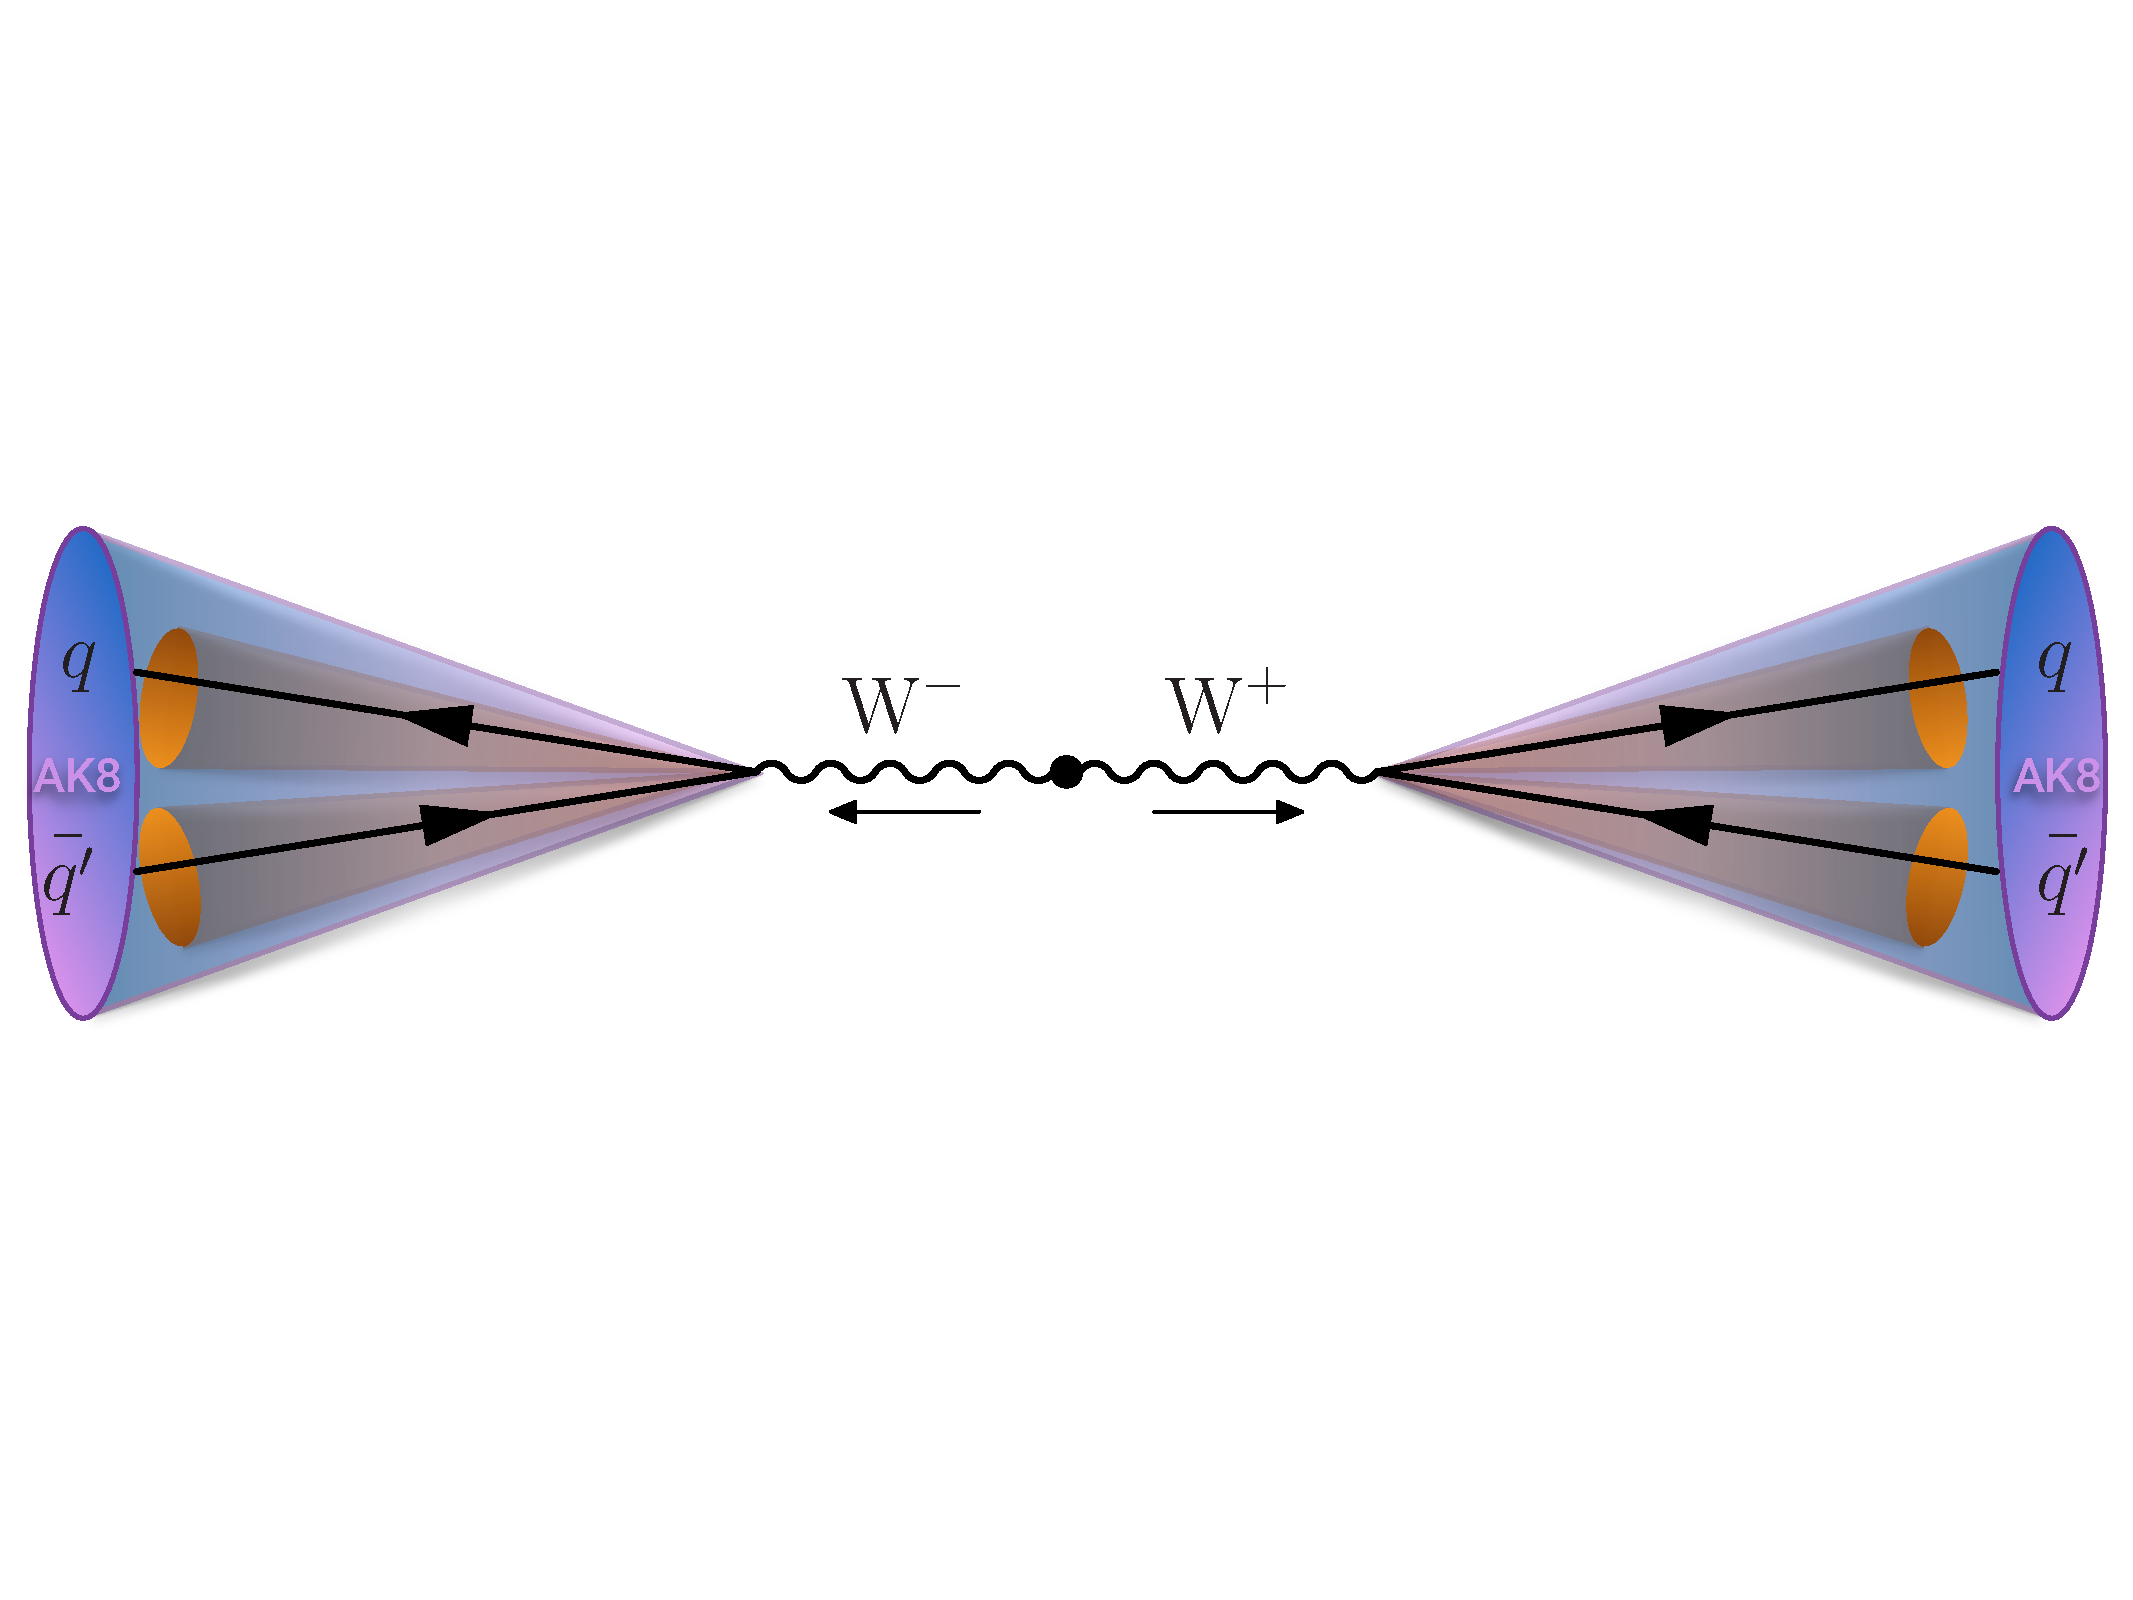
\includegraphics[width=\columnwidth]{figures/WWqqqq_merged.pdf}
\caption{If a heavy (> 1 TeV) resonance decays into vector bosons, the transverse momentum of each boson will be large and its decay products are merged into one single large  jet.}\label{Fig1}
\end{center}
\end{figure}
The two jets are each expected to have a mass around the W or Z boson mass, and some intrinsic substructure stemming from their two-pronged decay. The invariant mass of the dijet system, $m_{jj}$, should be roughly equal to the resonance mass $m_X$. This dijet system is the final state under scrutiny and the dijet invariant mass is the parameter of interest. The main background for such an analysis is QCD multijet events. Quark/gluon jets can obtain a high mass due to diffuse radiation, and QCD processes have such a large cross section that the number of QCD jets with a mass compatible with the W mass can be large. In order to discriminate between the two, we take advantage of three properties. First, the true mass of signal and background jets should be very different. Second, signal jets should appear two-prong like, as opposed to quark/gluon jets. And third, the dijet invariant mass for the signal process should peak around the resonance mass while the QCD spectrum is predicted to be a smoothly falling distribution. The strategy therefore consists of performing a smoothness test on $m_{jj}$ of the observed data; a so-called "bump-hunt", by assuming that the signal will appear as a bump on top of a smooth distribution.
% This is illustrated in Fig.~\ref{Fig2}.
%\begin{figure}[h!] 
 %   \centering
  %  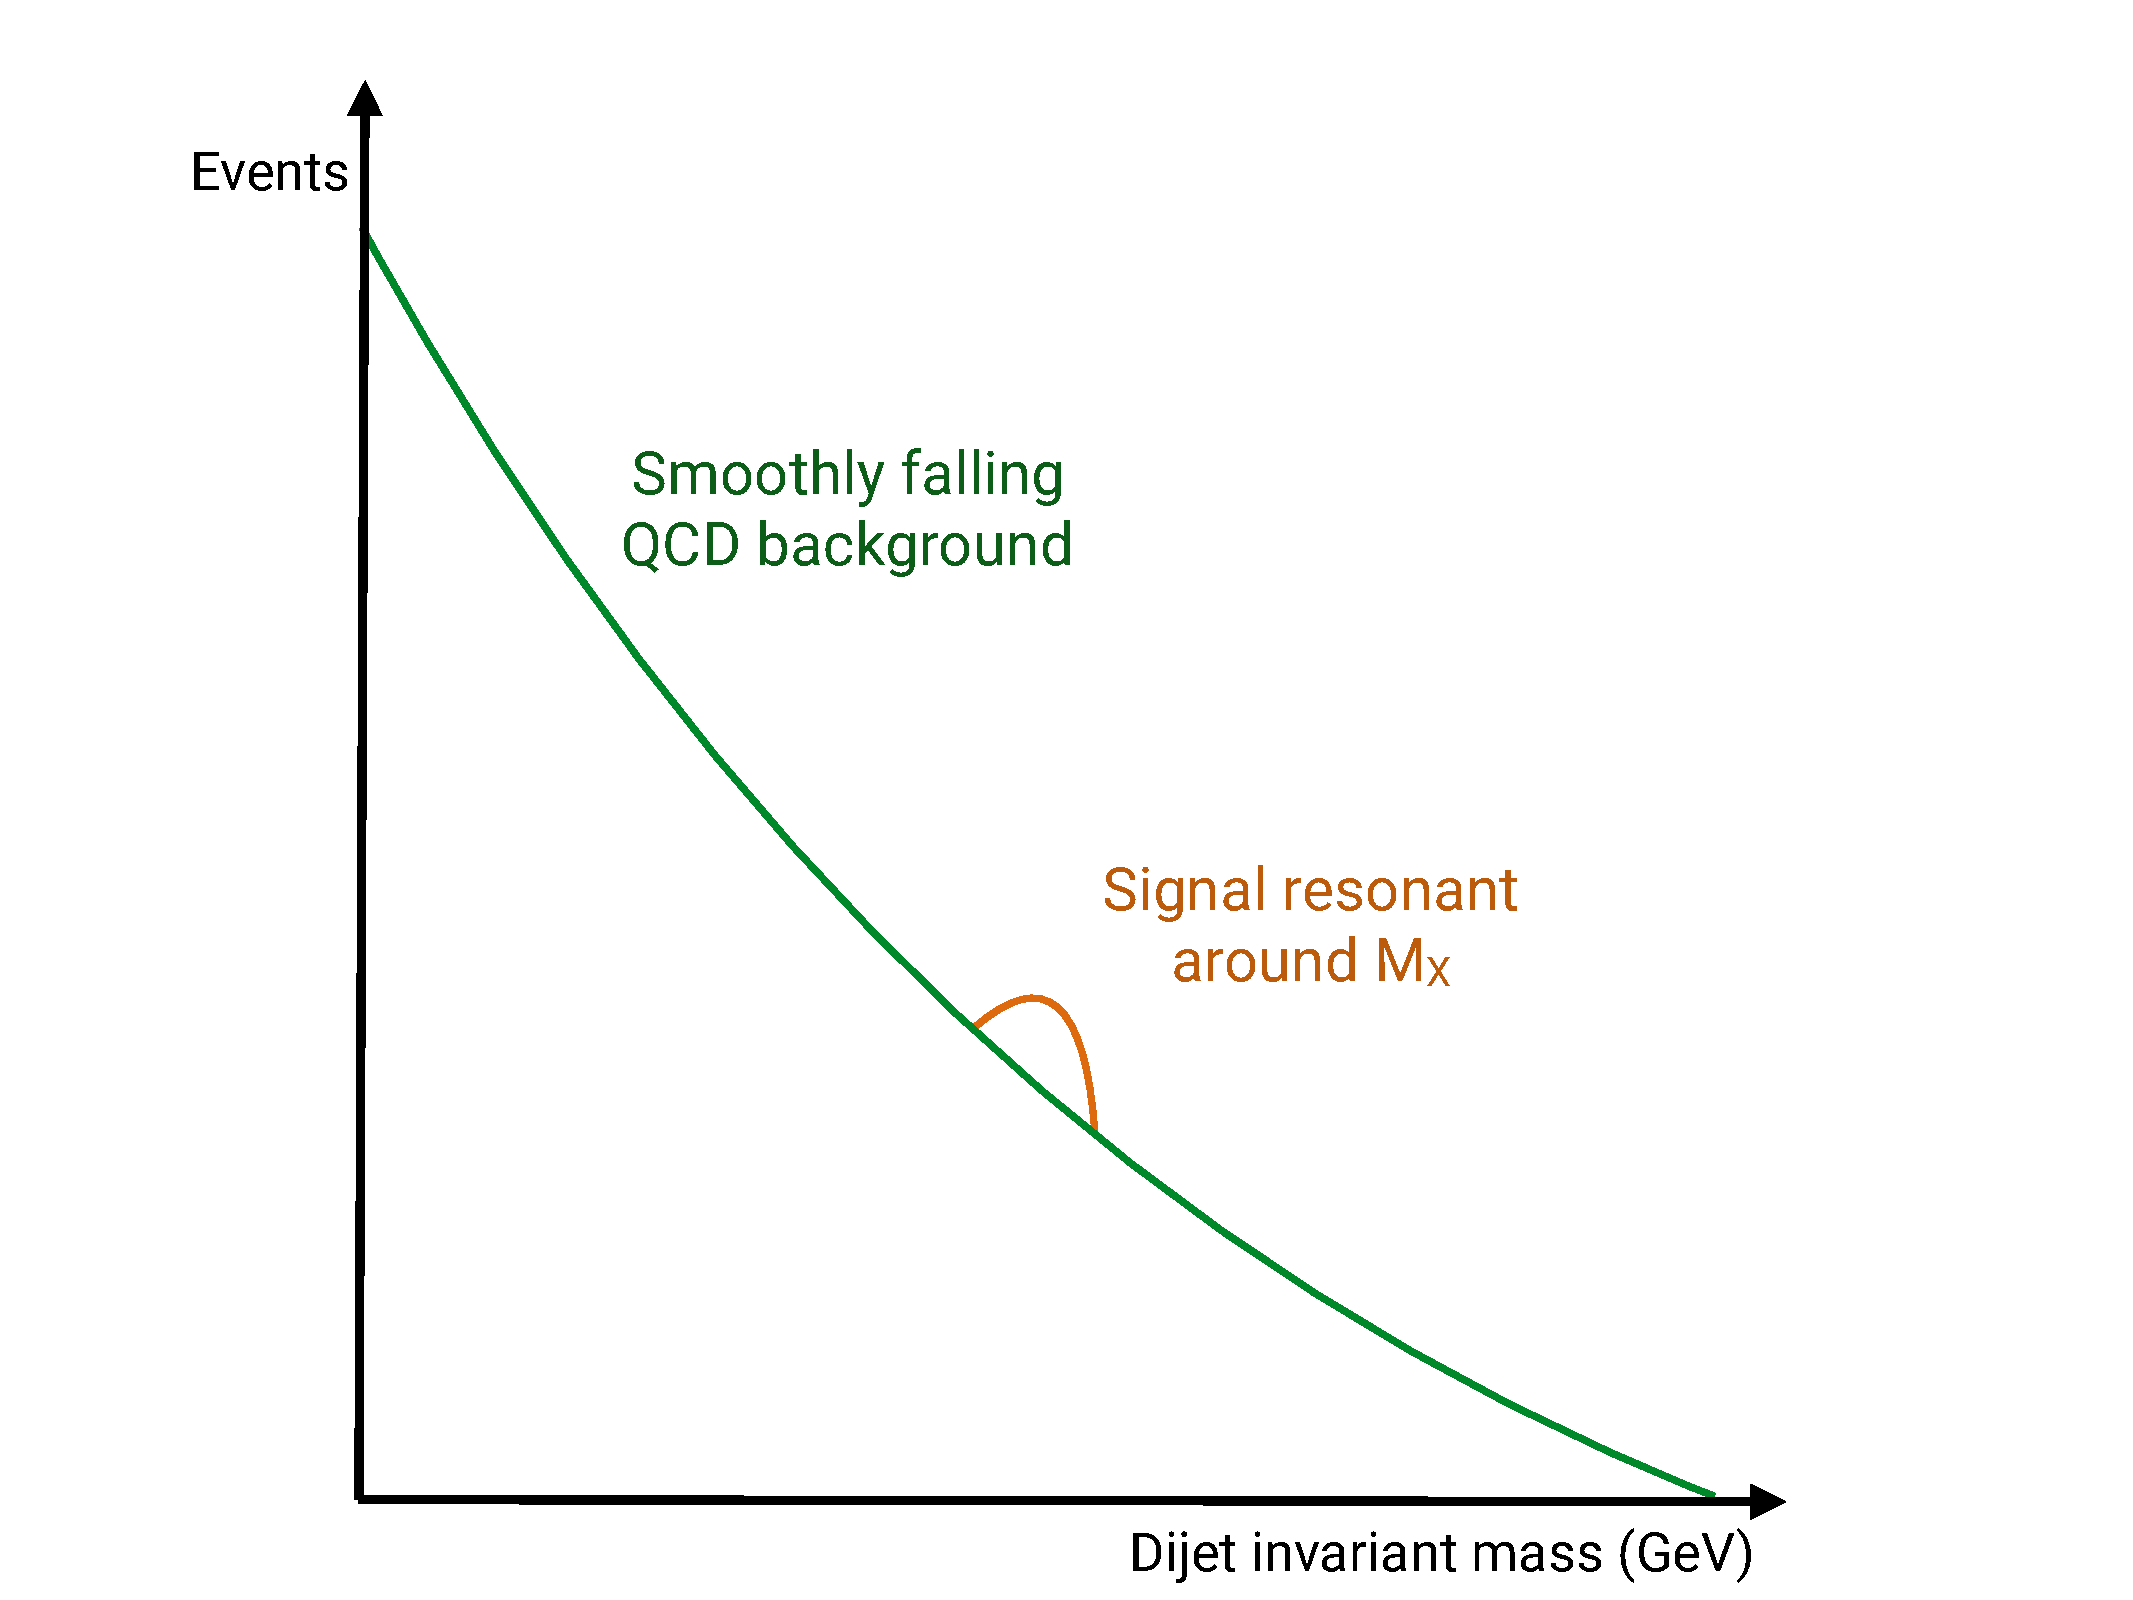
\includegraphics[width=0.79\columnwidth]{figures/sigExtraction.pdf}
    %\caption{The search strategy consists of looking for signal "bumps" in the dijet invariant mass on top of a smoothly falling QCD multijet background.}  
    %\label{Fig2}
%\end{figure}
The benefit of such a method is that there is no need for a simulation of the background, a necessary advantage as Monte Carlo with $\sqrt{s}=13$ TeV and had never before been validated.

I was the sole analyst running a full analysis of the first 13 TeV data collected in 2015, and managed to bring the search to a published results~\cite{Sirunyan2017} within 5 months of data taking, as one of the most anticipated results with the new dataset due to the previous excess. It became one of the first 13 TeV results ever published, and one of the two first "boosted" searches to be performed at 13 TeV at CMS. The search set the most stringent limits on the signal hypotheses under scrutiny to date.

\section{Developing a pileup-resistant and perturbatively-robust vector-boson tagger}
\label{sec:yearII}

After publishing the analysis of the full 2015 data set, I looked towards 2016. In this year, CMS would collect 10 times more data, but at the cost of a higher mean number of interactions per proton bunch crossing, causing additional interaction vertices per event (pileup) whose effect would need to be mitigated in order to maintain analysis sensitivity. I had become very much involved with jet algorithms in CMS and wanted to explore better algorithms intended to distinguish hadronically decaying vector bosons from jets originating from quark and gluons; and one promising direction was exploring a new pileup-removal algorithm called Pileup per particle identification (PUPPI)~\cite{Bertolini2014}. PUPPI had proven itself far superior to the current pileup-removal algorithm in terms of jet observables, like the jet mass, for large radius jets. Another promising new algorithm to explore was Soft Drop~\cite{Larkoski:2014wba}, intending to improve the vector-boson mass resolution and better discriminate it against quark/gluon jets by removing soft radiation from the jet. Algorithms intended to improve the jet mass resolution by removing radiation from the jet are referred to as "jet grooming algorithms", and the benefit of softdrop was that it had certain favorable theoretical qualities: the softdrop algorithm, in addition to removing sensitivity to the soft divergences of QCD as all grooming algorithms do, eliminates all correlated soft emissions in the jet, leading to no non-global logarithmic terms (NGLs) in the jet mass~\cite{Dasgupta:2013ihk}. NGLs arise from configurations where, for instance, a soft gluon is radiated into the jet cone, as illustrated in Figure~\ref{Fig3}. 
\begin{figure}[h!]
\centering
 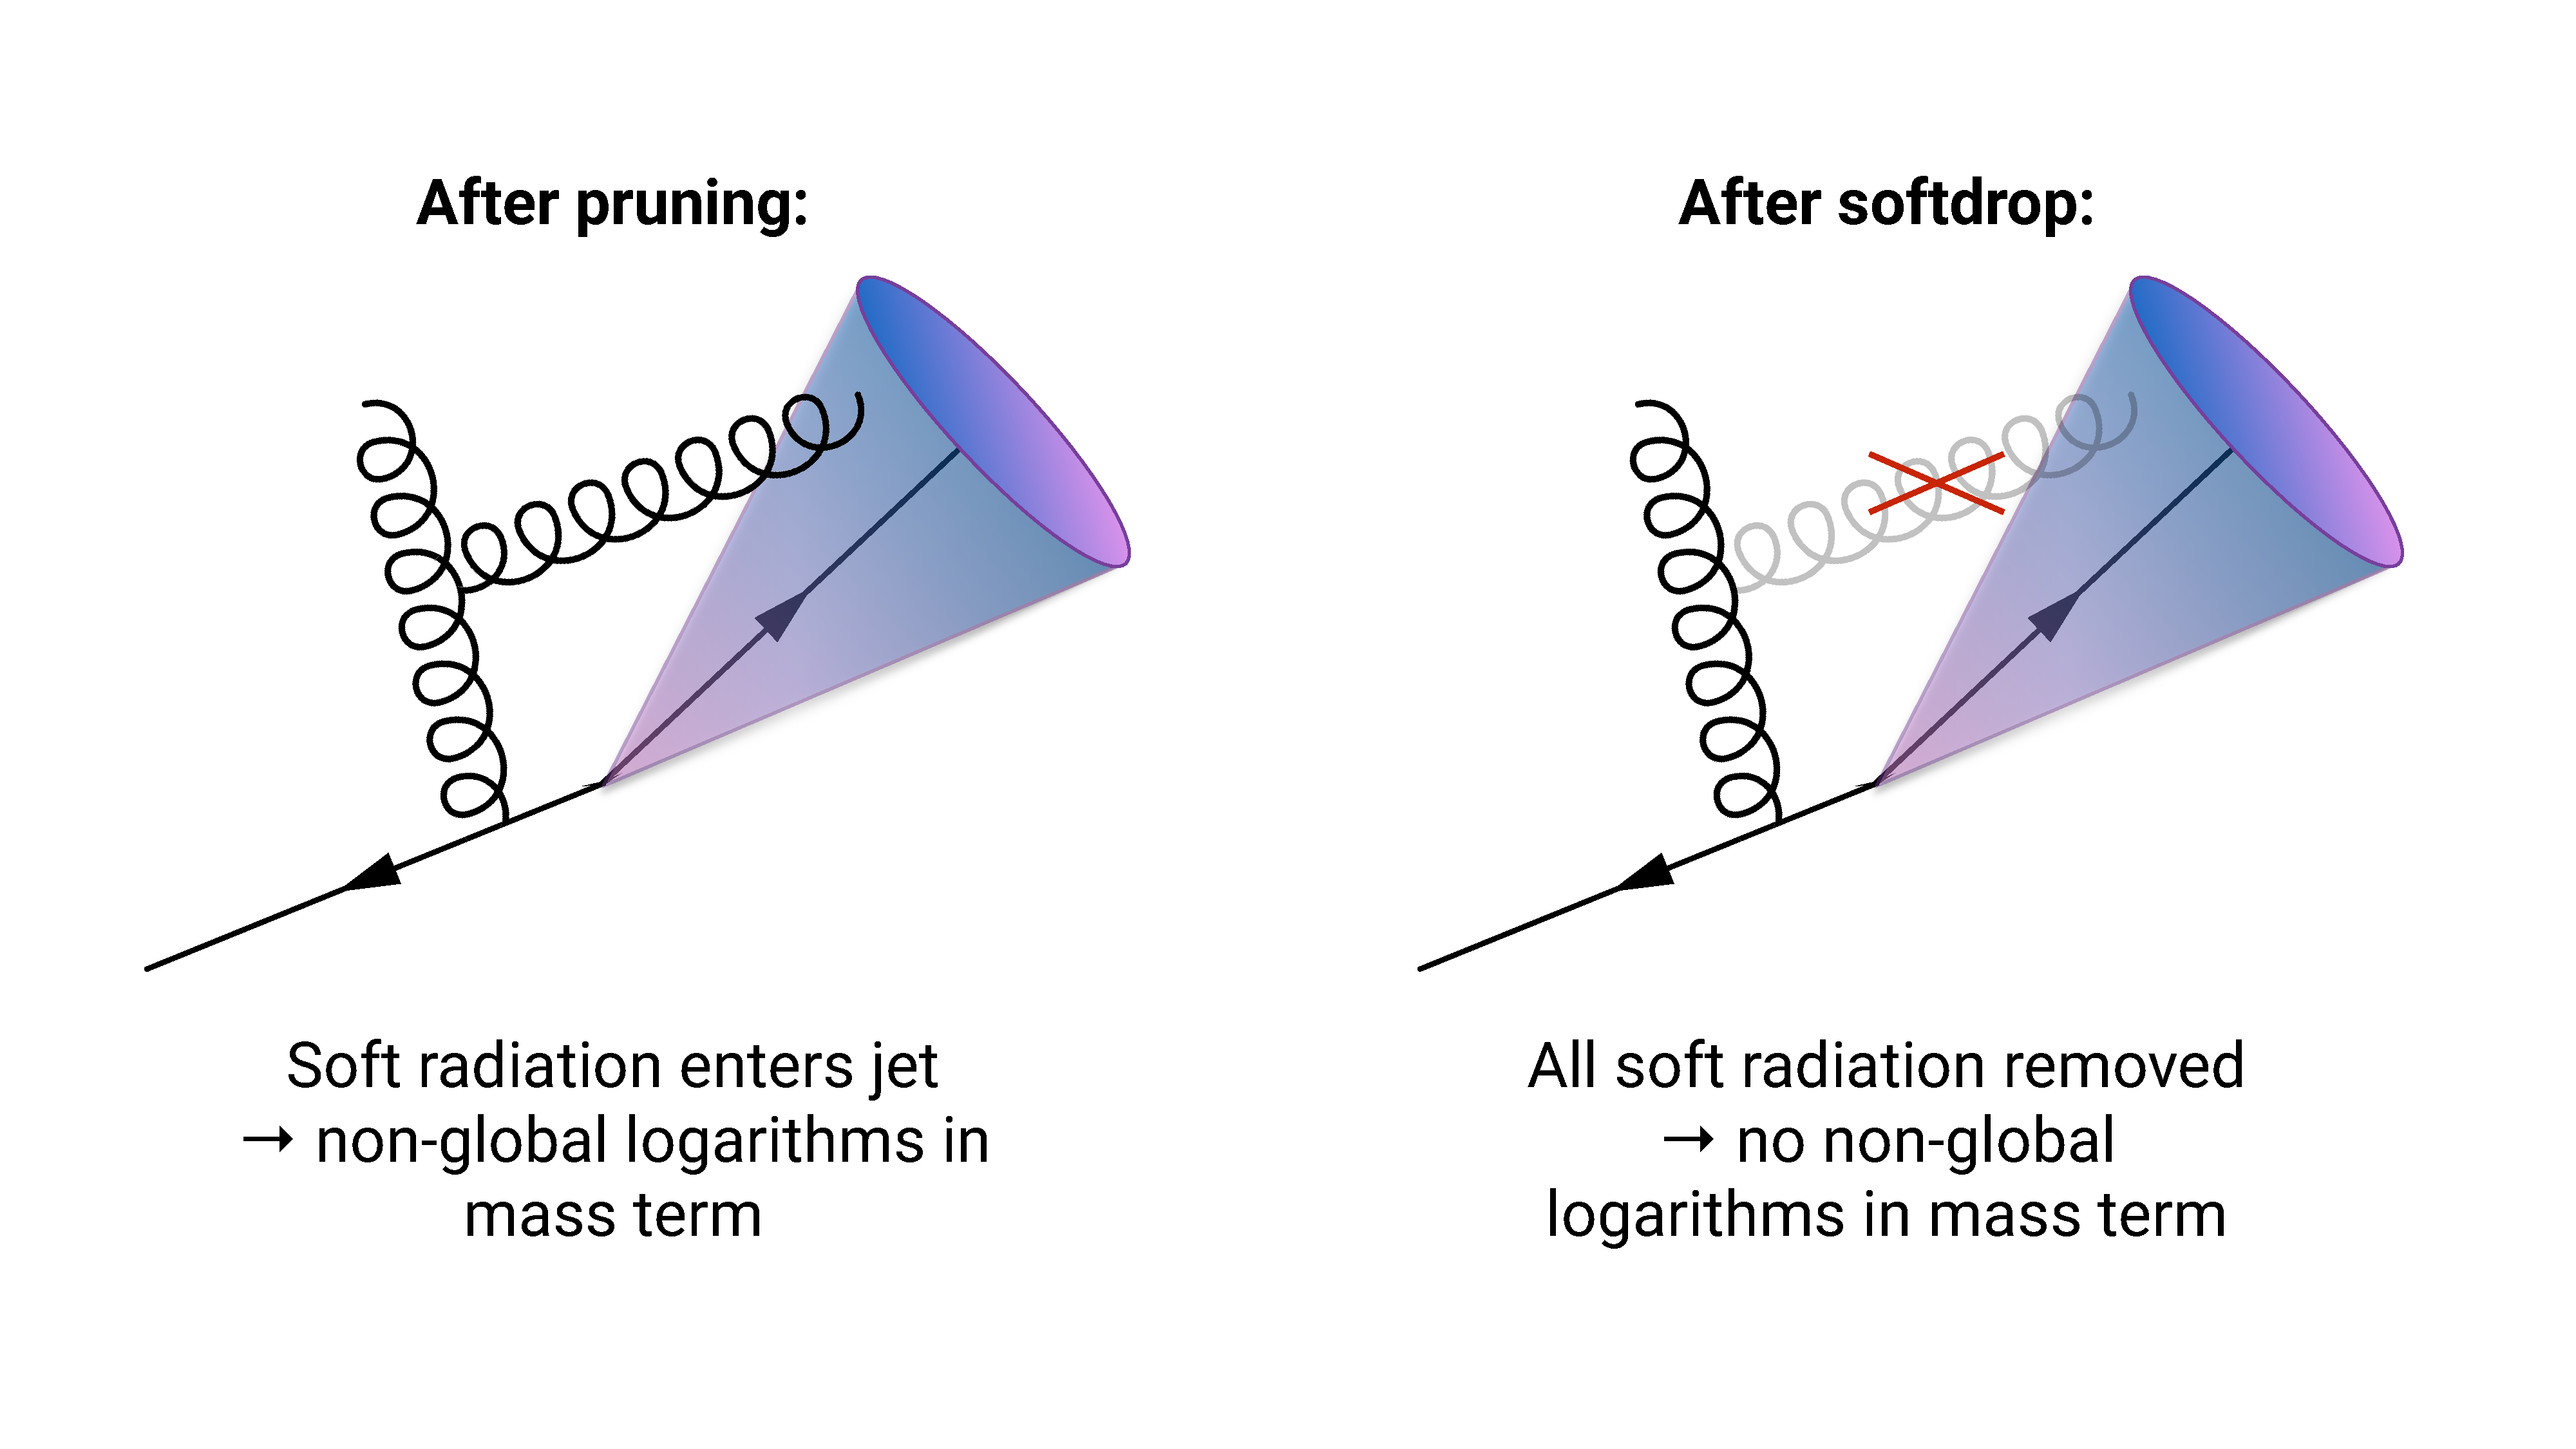
\includegraphics[width=\columnwidth]{figures//ngls.pdf}
\caption{The pruning algorithm does not remove all soft emission and therefore has non-global logarithmic terms in the jet mass. The softdrop algorithm removes all soft emissions and is free of non-global logarithms.}
\label{Fig3}
\end{figure}
The benefit of being NGL-free, is that one can calculate the softdrop jet mass to a significantly higher precision than what is possible for other grooming algorithms or for the plain jet mass (NGLs are the main reason a full resummation of the plain jet mass beyond NLL accuracy does not exist). There were therefore theoretically well-motivated reasons for wanting the baseline CMS vector-boson tagger to be softdrop-based.

I therefore optimized, commissioned and validated a new vector-boson tagging algorithm, with the goal of a more robust and theoretically well motivated tagger for all future analyses in CMS using vector-boson tagging~\cite{CMS-PAS-JME-16-003}. This included the derivation of dedicated jet-mass corrections for this new type of jets (jets after PUPPI and softdrop have been applied) to account for detector effects that can affect the observed jet mass, and depend on the jet \PT and pseudo rapidity $\eta$. The W-jet mass mean as a function of jet \PT and $\eta$ before (left) and after (right) corrections, is shown in Fig.~\ref{Fig3}.
\begin{figure}[h!]
\centering
 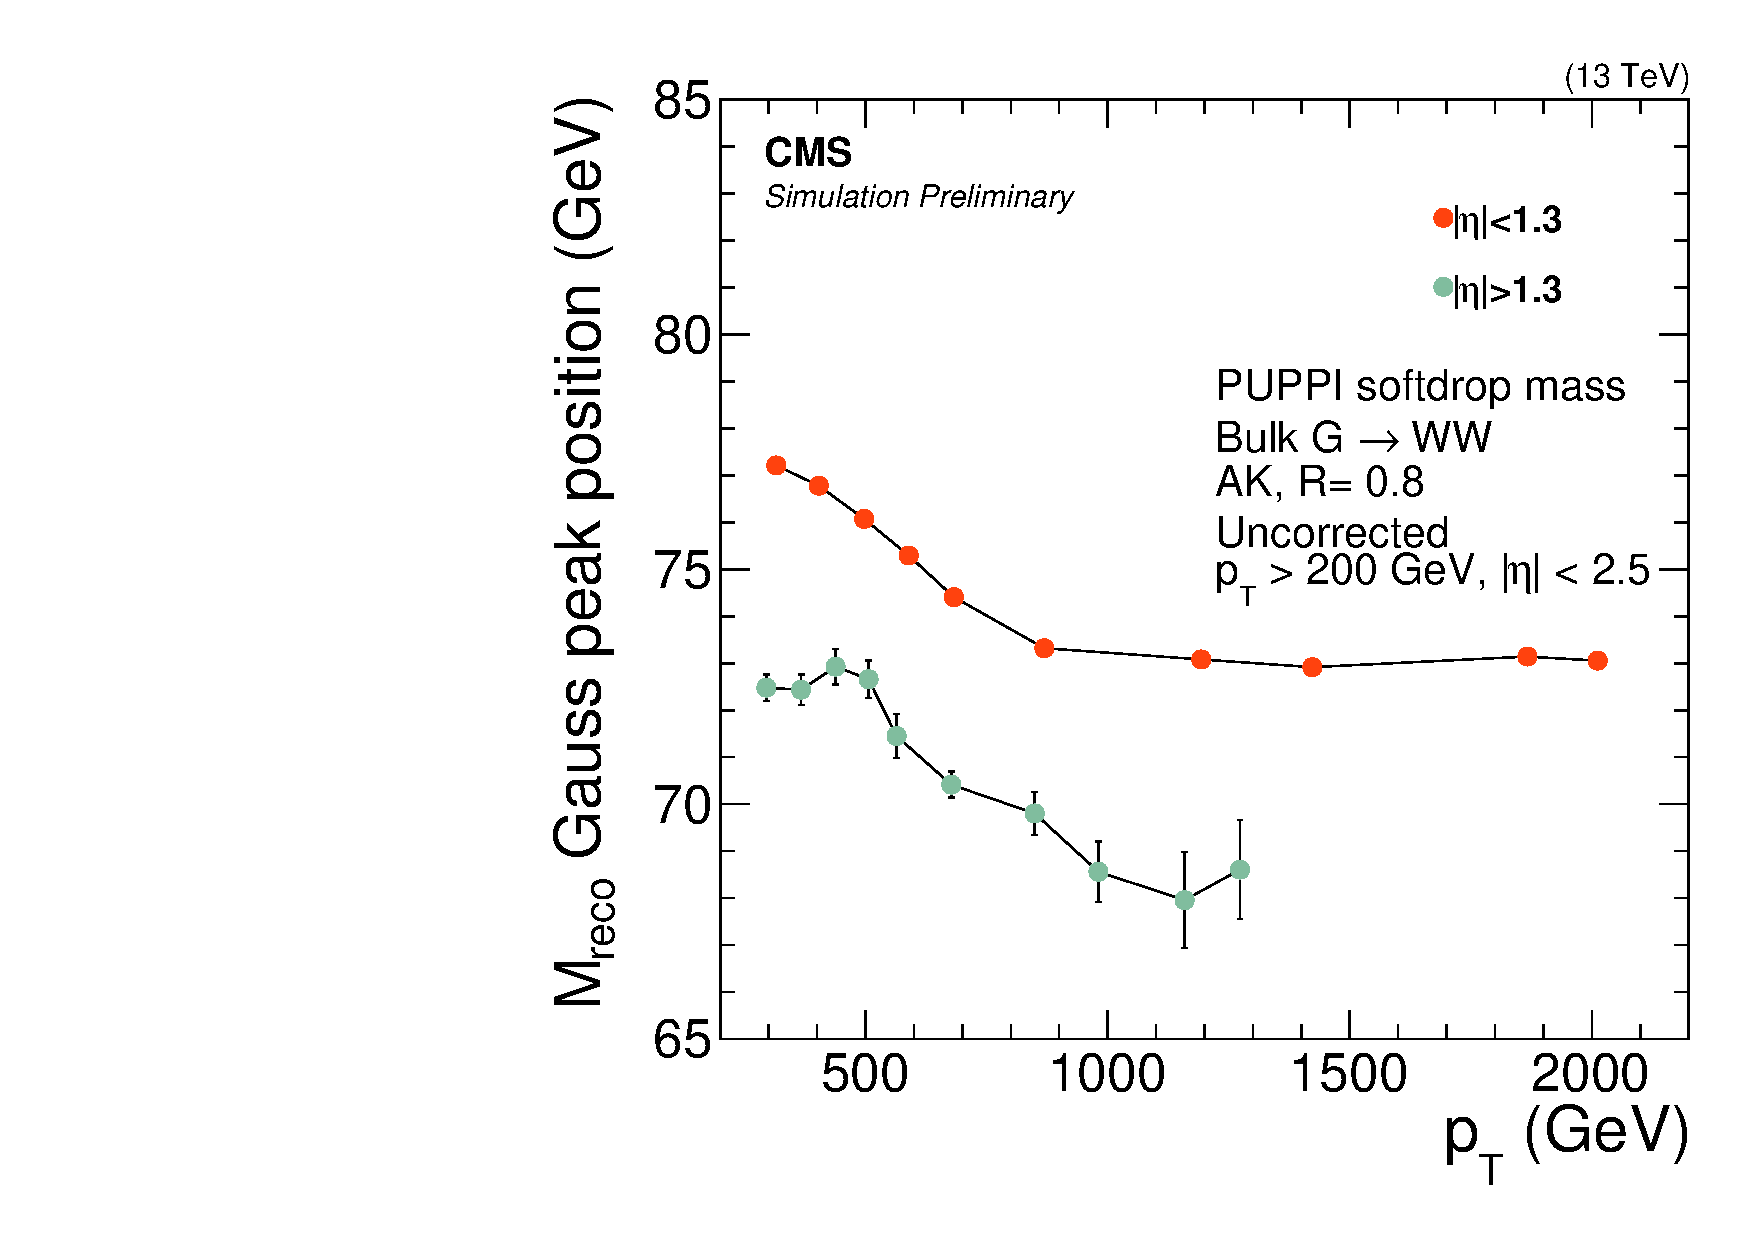
\includegraphics[width=0.49\columnwidth]{figures/RecoPuppiSoftdropMass_vspt.pdf}
  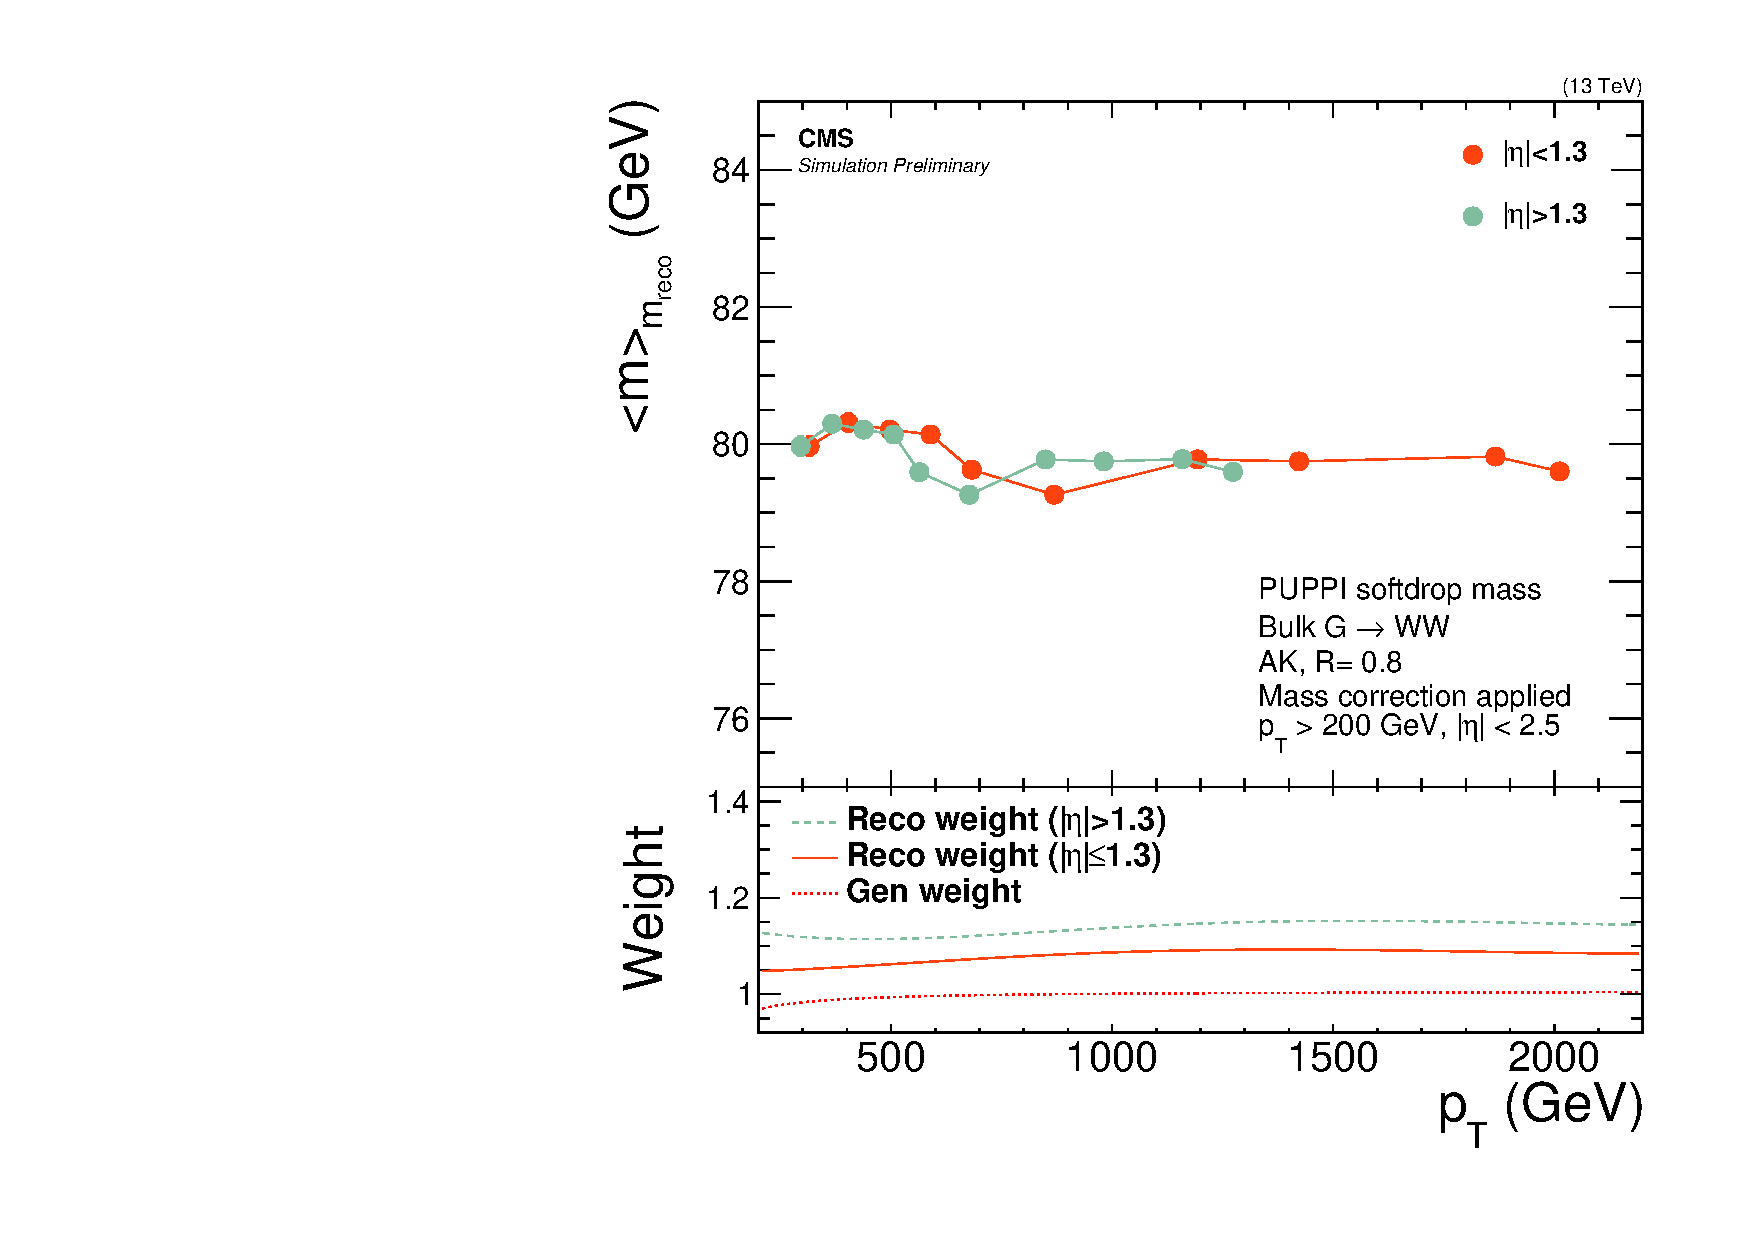
\includegraphics[width=0.49\columnwidth]{figures//ClosureTest_RecoMass.pdf}
\caption{The Gaussian mean of the fitted jet softdrop mass for W-jets before (left) and after (right) dedicated jet mass corrections have been applied as a function of jet transverse momentum. }
\label{Fig3}
\end{figure}
I published an analysis of the data collected in 2016 as the first analysis to take advantage of this new vector-boson tagging algorithm that I developed~\cite{CMS-PAS-B2G-16-021,Sirunyan:2017acf}, an algorithm (with corresponding jet mass corrections) that afterwards became the default vector-boson tagging algorithm in CMS. More than 20 subsequent CMS analysis take advantage of the tagger and jet mass corrections (these are listed in my attached publication list). In parallel, I developed efficiency scale factors to account for any mismodeling in simulation that affect the tagging efficiency, both for the newly developed tagger, and for the previous default tagger. These are the CMS recommended scale factors for any analysis using vector-boson tagging, and I evaluated these for data collected throughout years 2015, 2016, and 2017 ( full analyses in their own right requiring months of dedicated work). These scale factors are crucial for a correct signal yield estimation. The published analysis, in addition to introducing a novel tagging algorithm, also included a brand new search: a search for excited quarks decaying to a quark and a vector boson. This was an extremely interesting search attempting to probe whether quarks truly are fundamental particles or not, by checking whether a collision could excite a quark to a higher energy state, leaving its constituents the same, but with a higher mass. It was the very first time such a search in this channel was performed at 13 TeV~\cite{CMS-PAS-B2G-16-021}. No significant deviations from the  Standard Model prediction were observed in either of the searches, leading us to exclude non-SM resonances decaying to VV (where V=W/Z) or qV up to very high masses, $\sim3$ TeV for VV signals and $\sim5$ TeV for qV signals.

\section{A novel multi-dimensional signal extraction framework}
\label{sec:yearIII}
No excesses had been observed in analyses of the 2015 and 2016 data sets described above. For my next project I therefore wanted to look beyond standard signal hypotheses by establishing a method to efficiently probe a large range of different signal hypotheses. There could still be signal present in our data, but it might look slightly different than what we had assumed up until now. For instance, new signals could exist where the observed jet mass is slightly different than that of a W/Z boson mass. Further, these could be 4-pronged objects rather than 2-prong, which would cause the excess to vary in size depending on the analysis-specific, vector-boson tagger in use. This is illustrated in Figure~\ref{Fig4}.
\begin{figure}[h!]
\centering
 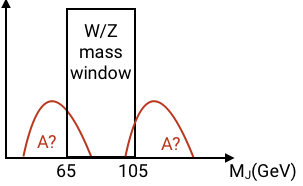
\includegraphics[width=0.49\columnwidth]{figures/tails.png}
 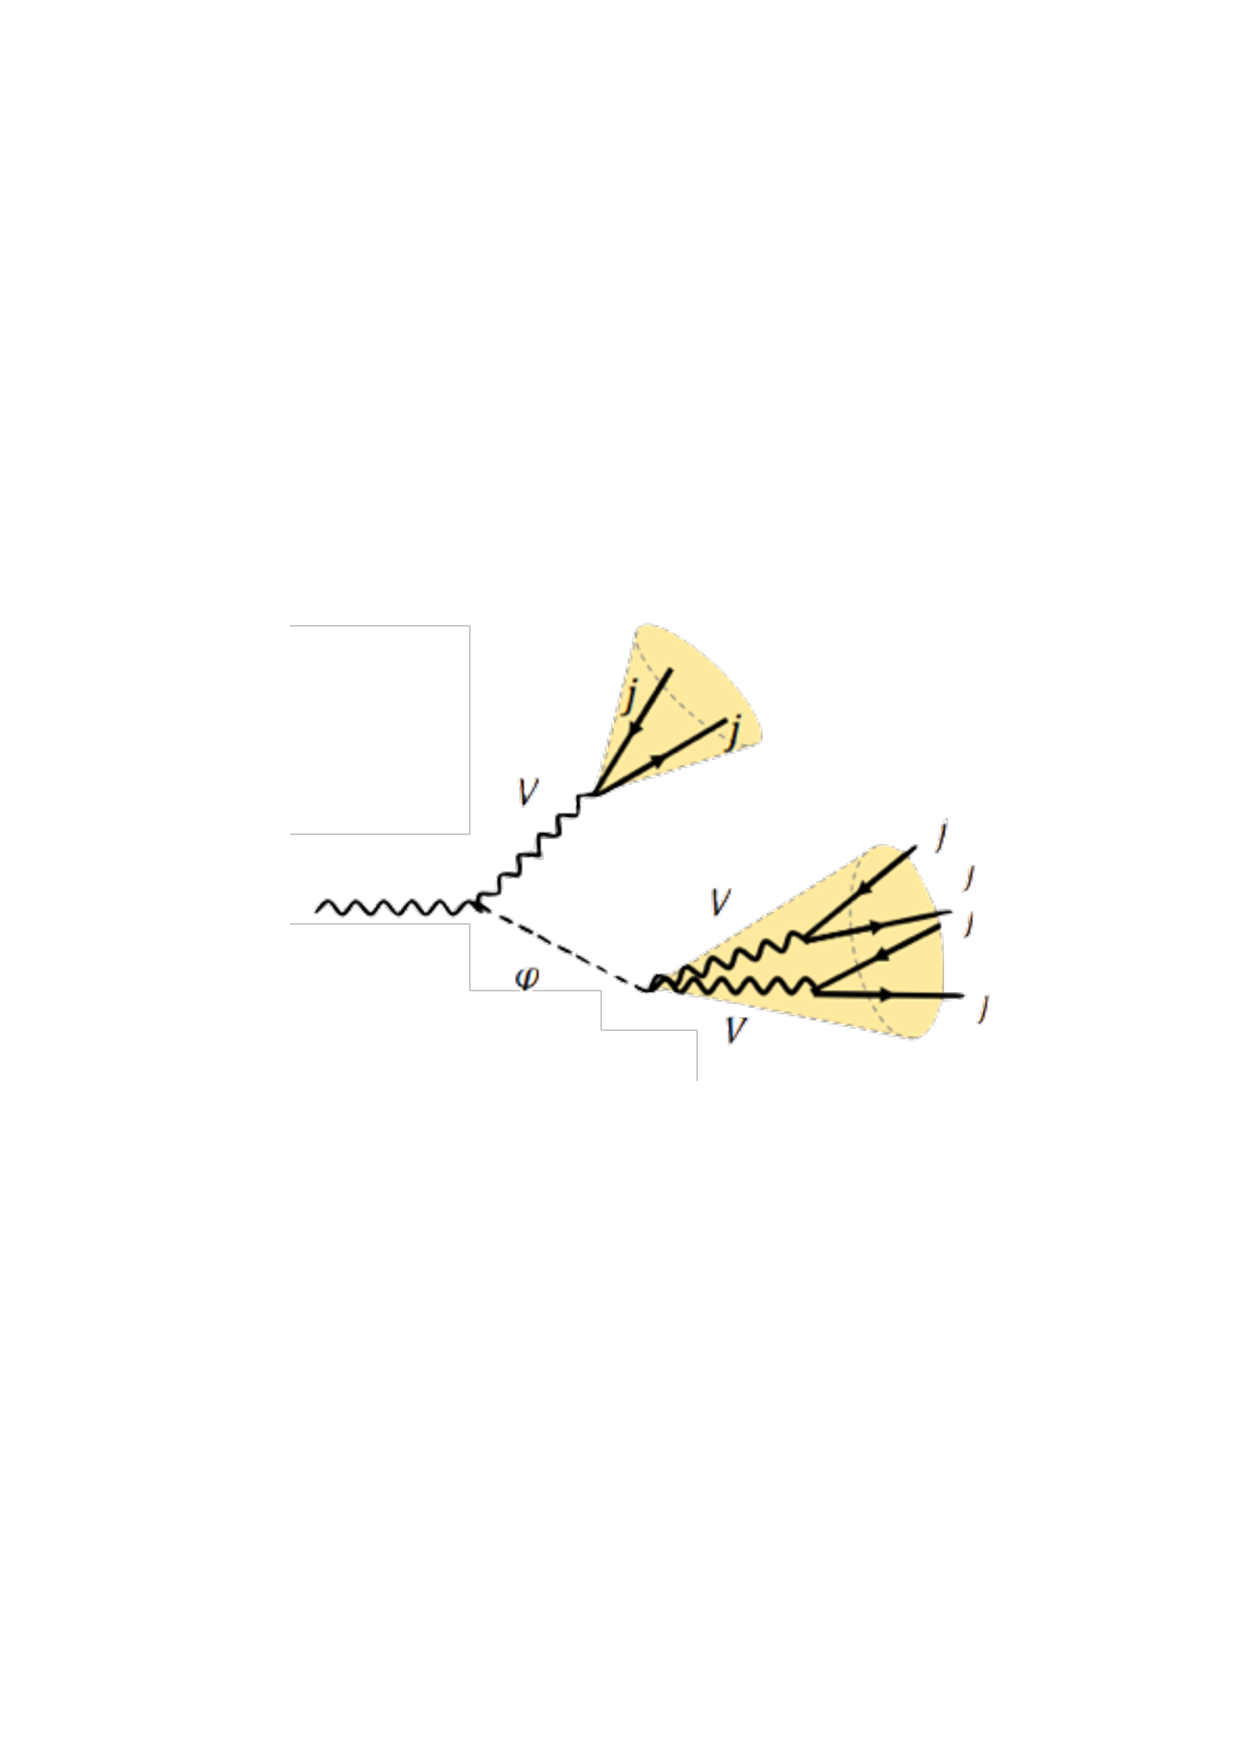
\includegraphics[width=0.49\columnwidth]{figures/triboson2.pdf}
\caption{New signals that peak at a mass slightly different than the W/Z mass (left) and have a slightly different substructure (right) could be present in our data.}
\label{Fig4}
\end{figure}
In order to efficiently search for any signal peaking in the jet mass, we decided to build a generic framework that would allow searching for peaks anywhere in the jet mass and dijet invariant mass spectrum.
Rather than selecting jets with a jet mass compatible with the W/Z boson mass and searching for resonances peaking in the dijet invariant mass, we would attempt to look for resonances peaking anywhere in the hyperplane formed by the mass of each jet and their dijet invariant mass, scanning the full mass spectrum in a single analysis, as illustrated in Fig.~\ref{Fig5}. We would first demonstrate the new method in the context of the diboson all-hadronic search, which would allow for a straight forward comparison of the obtained results.
\begin{figure}[h!]
\centering
 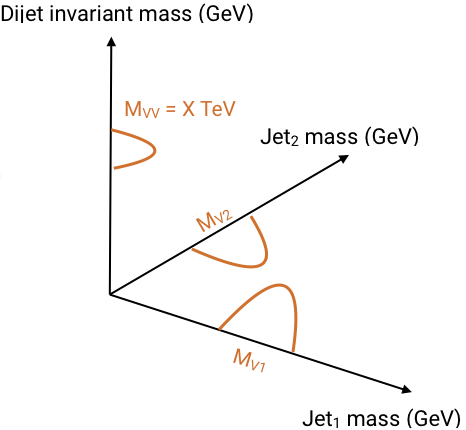
\includegraphics[width=0.49\columnwidth]{figures/3D.png}
\caption{With the new multi-dimensional fit method, the signal is extracted from the $m_{\rm{jet1}}$-$m_{\rm{jet2}}$-$m_{\rm{jj}}$ hyperplane, where it peaks in all three dimensions.}
\label{Fig5}
\end{figure}
The benefits of doing a multi-dimensional fit is that we can search for resonances decaying to VV (V=W/Z), VH (H=Higgs), HH, VX, VH, XX, or XY, where X and Y are new hypothetical bosons, in the same analysis. Additionally, a jet-mass selection is no longer needed as we fit the full jet mass line-shape to extract the signal. This effectively increases the signal statistics since a large fraction of the W/Z signal falls outside the mass window (20\%). Fitting the groomed-jet mass and resonance mass together also allows for the addition of nuisance parameters that simultaneously affect both in order to fully account for the correlation between the variables. Finally, we would model the background starting from simulation, rather than from a dijet fit to data. This allows the background shape to assume non-smooth distributions, and could allow the search to probe lower dijet masses. Replacing the parametric fit by a simulation-based model would also reduce the fit sensitivity to background fluctuations in the extreme tails of the dijet invariant mass spectrum. However, this technique would be challenging to implement, and require new techniques, such as Gaussian kernels with a mean and width obtained through forward-folding rather than single points in order to model the backgrounds, to be incorporated. We decided to re-analyze the 2016 data set in order to directly compare the sensitivity between the previous method and the multi-dimensional technique, as well as for the first time analyze the data collected in 2017.

For this search, I additionally optimized and commissioned a new vector-boson tagging algorithm intended to remove correlations between the tagger and jet \PT/mass (crucial for an analysis covering a large jet mass and dijet invariant mass range). It also provided a significantly higher signal sensitivity for our phase space.

Fig.~\ref{Fig6} shows the final fitted result and the data distributions projected onto two of the three dimensions of interest: the jet mass of one of the jets and the dijet invariant mass. Two beautiful peaks from the Standard Model Z(qq)+jets and W(qq)+jets background are observed. This is the first time these SM backgrounds have ever been measured in a diboson analysis. Their extracted cross sections are found to be compatible with the SM expectation~\cite{CMS-PAS-B2G-18-002}, a measurement made possible due to the nature of the fit and the optimized vector-boson tagging algorithm. The two peaks also allow us to constrain uncertainties affecting the signal yield, leading to a better analysis sensitivity.
\begin{figure}[h!]
\centering
 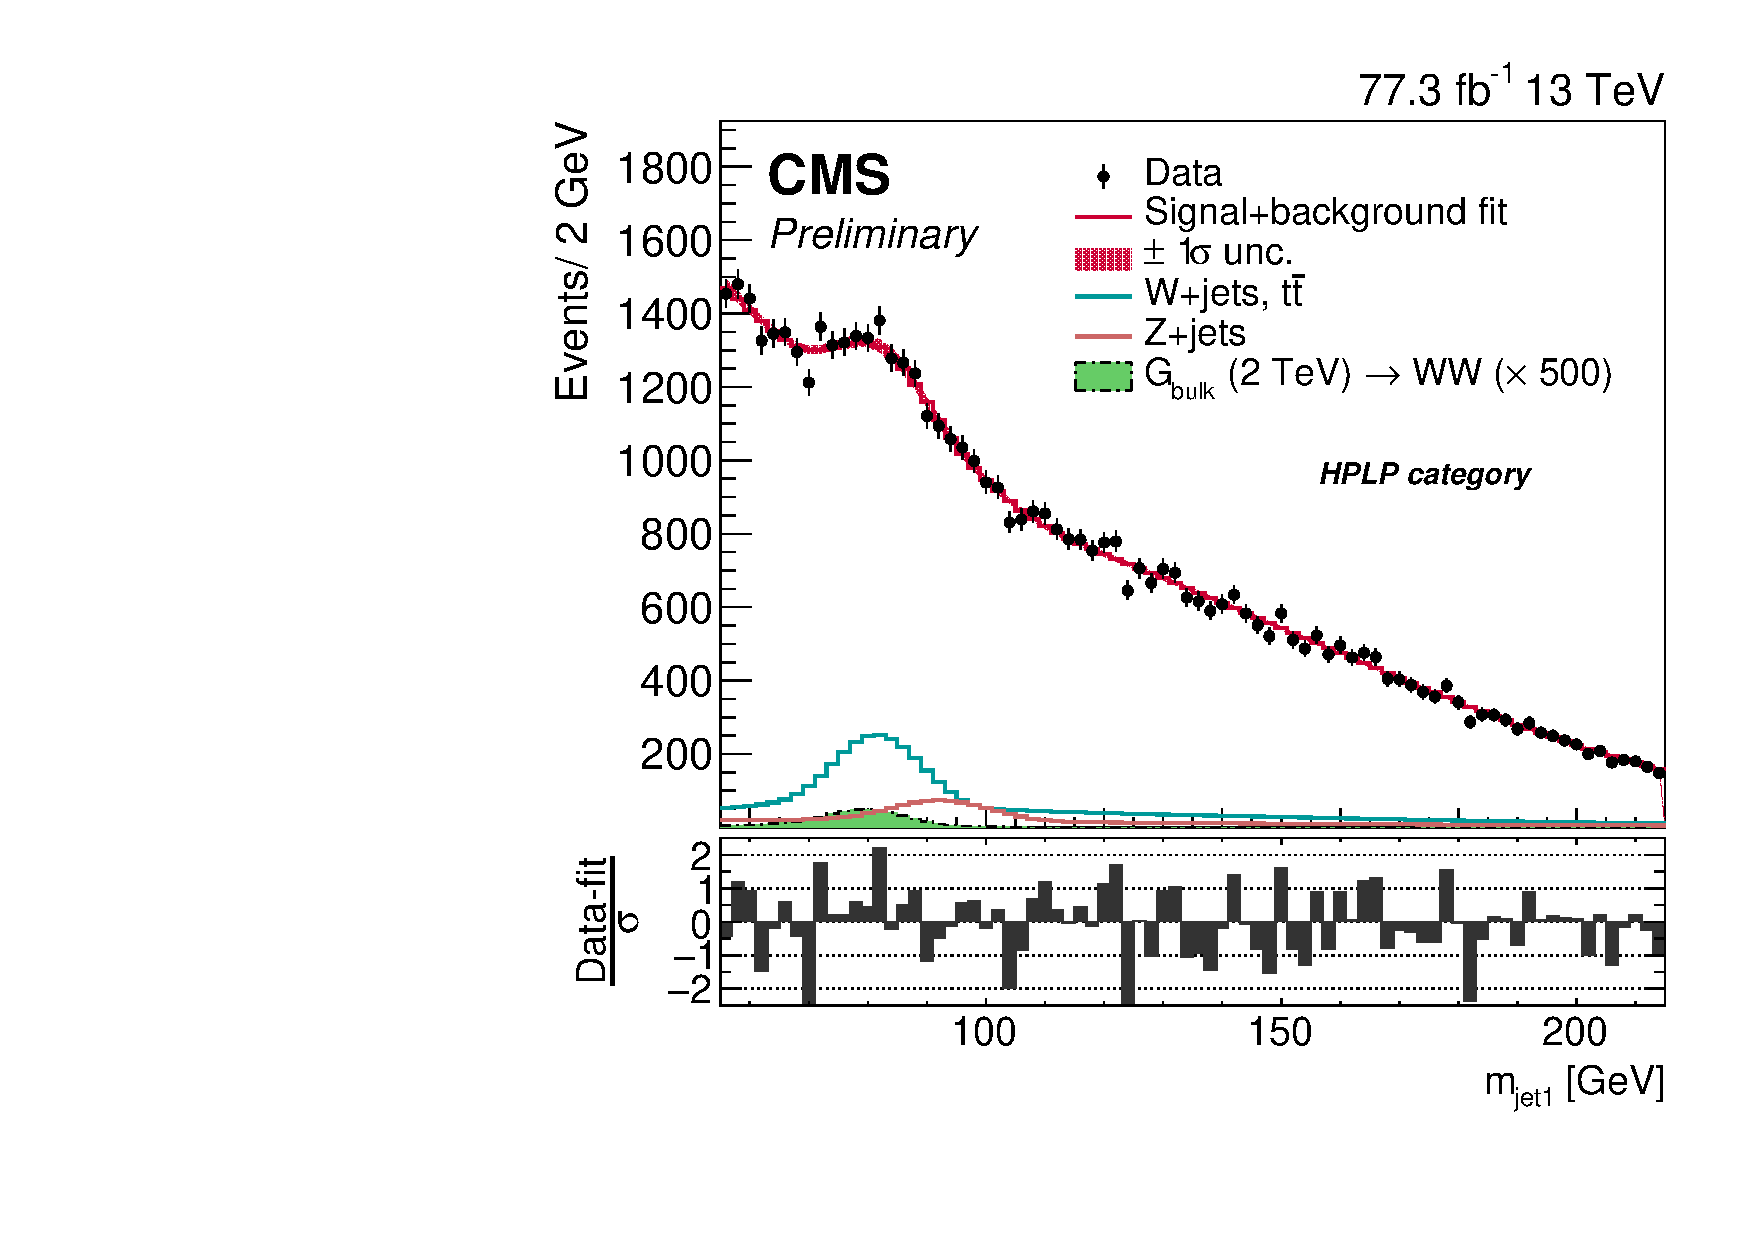
\includegraphics[width=0.49\columnwidth]{figures/PostFitComboHPLP_X-Proj__y___0_-1_z___0_-1_prelim.pdf}
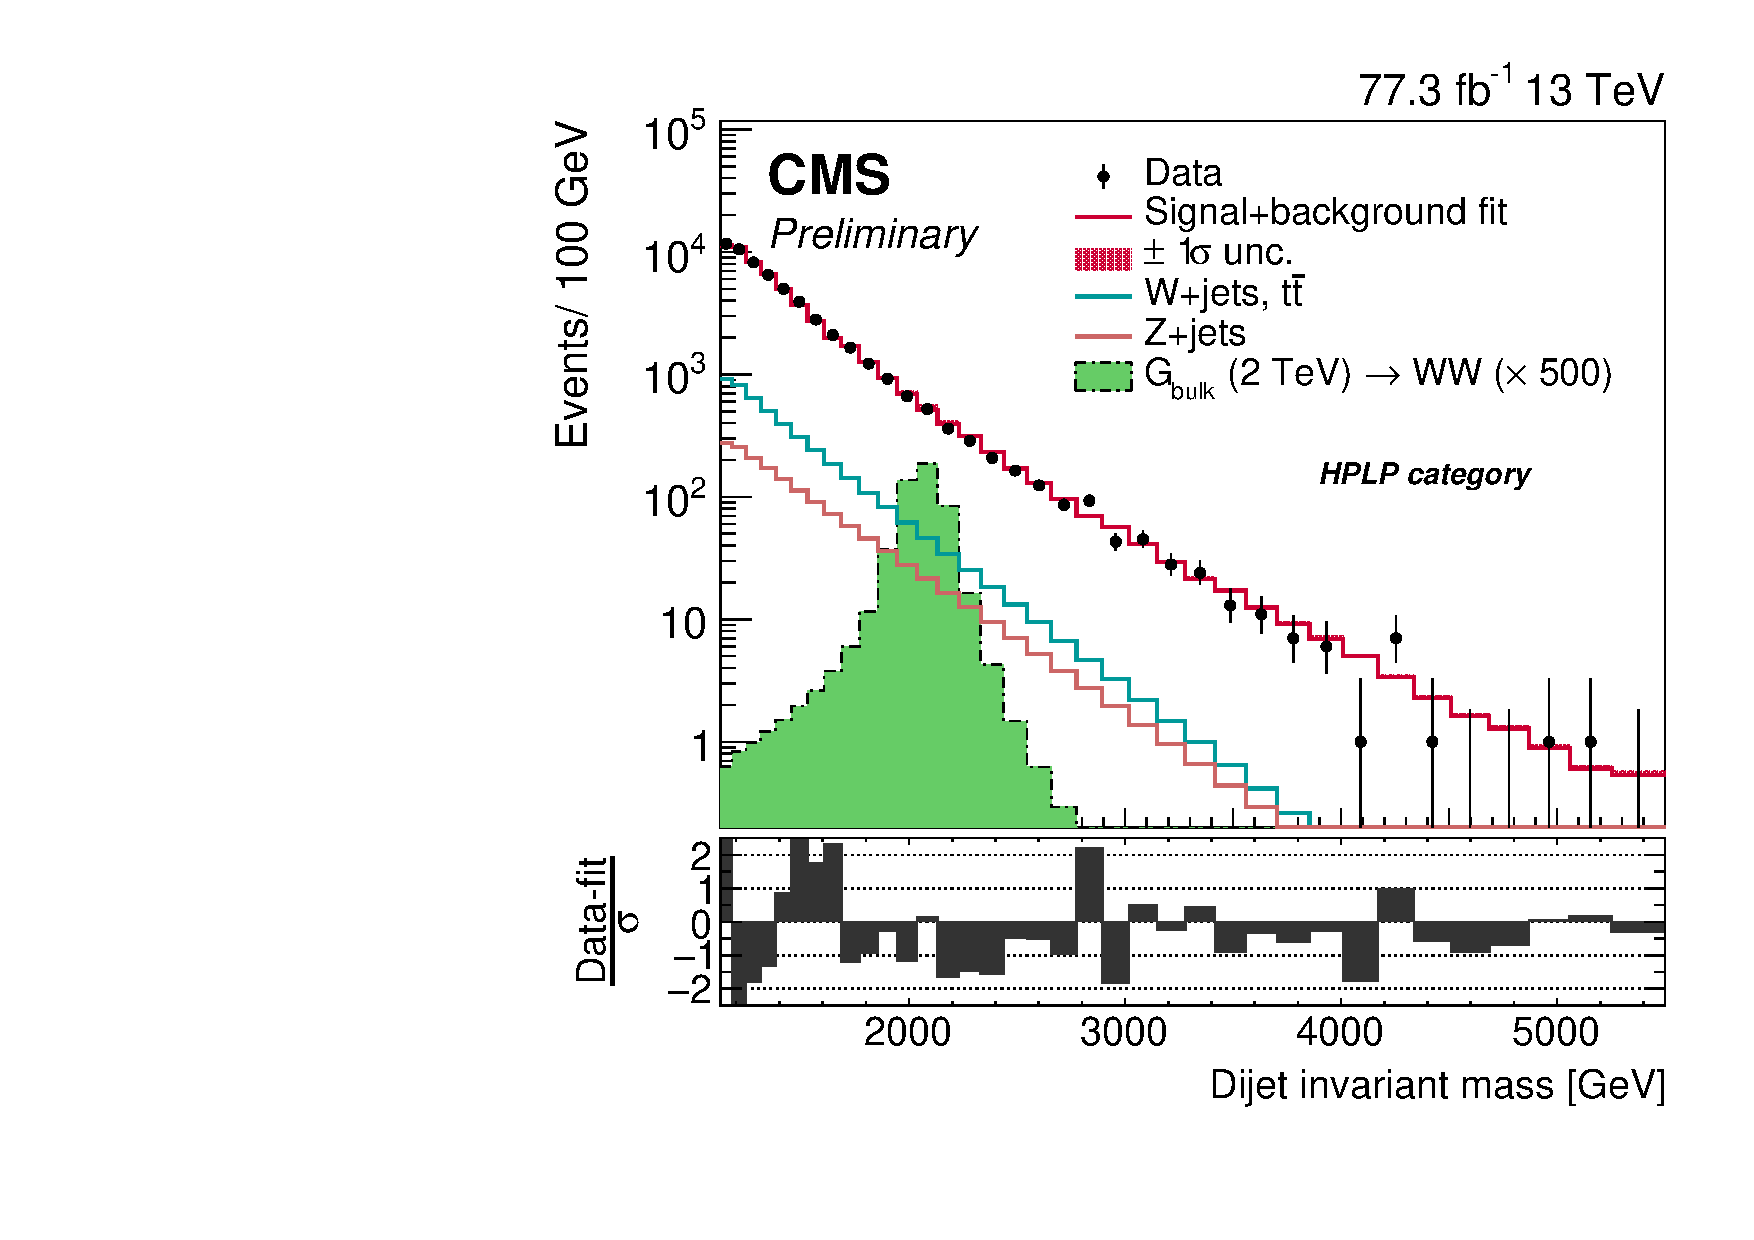
\includegraphics[width=0.49\columnwidth]{figures/PostFitComboHPLP_Z-Proj__x___0_-1_y___0_-1_prelim.pdf}
\caption{Comparison between the fitted result and data distributions for the jet mass of one of the jets (left) and the dijet invariant mass (right).  An example of a signal distribution is overlaid, using an arbitrary normalisation. Two beautiful peaks from Z(qq)+jets and W(qq)+jets are measured for the first time in diboson analyses.}
\label{Fig6}
\end{figure}
The obtained expected upper limits using the multi-dimensional fit method introduced here, can be compared to those obtained in the previous search described above using the same data set, Ref.~\cite{Sirunyan:2017acf}, in order to estimate whether there is a sensitivity gain in using the new method.
Figure~\ref{Fig7} shows the expected limits based on analyses of the data collected in 2016, either using the fit method presented here, or using the previous one-dimensional method. We obtain a 20-30\% improvement in sensitivity when using the multi-dimensional fit method, and about a 35-40\% improvement when combining the two data sets with respect to the individual results.
\begin{figure}[h!]
\centering
 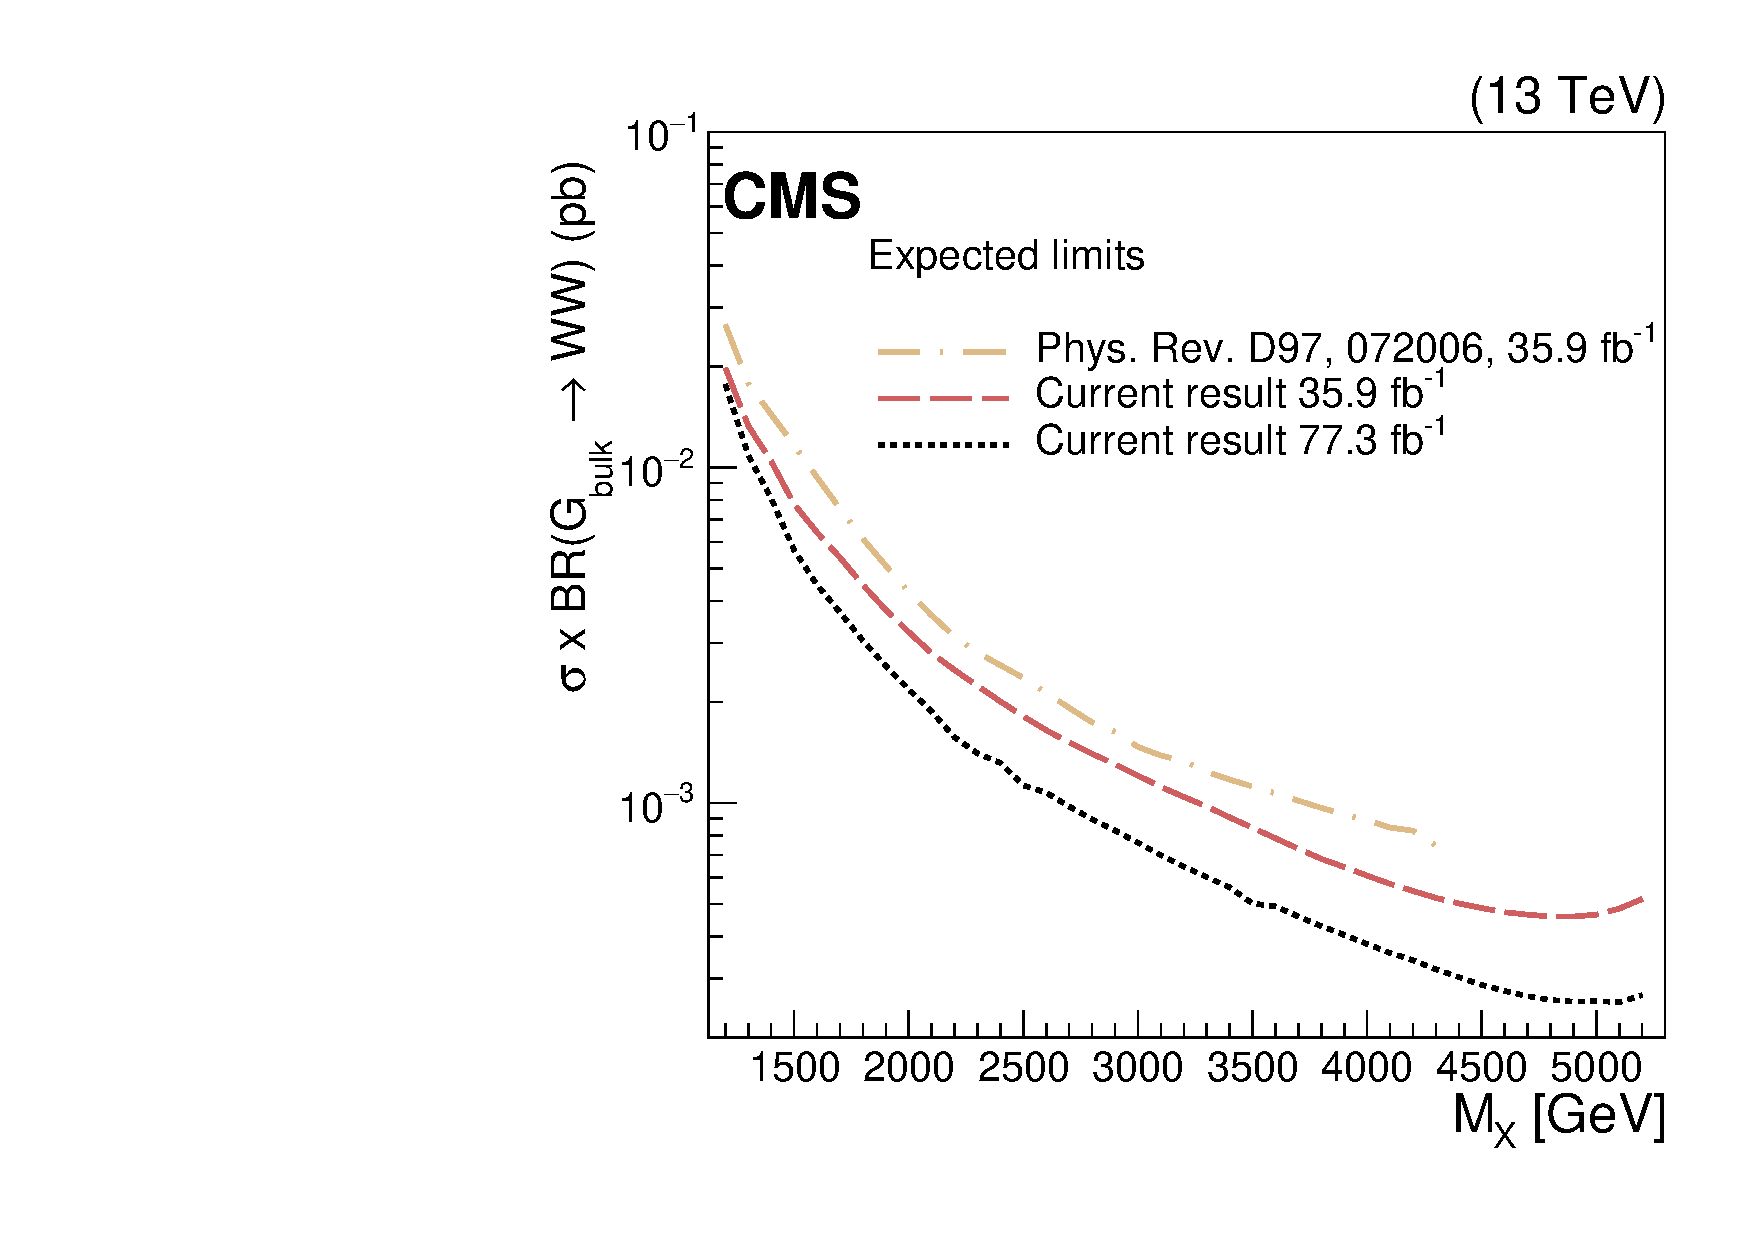
\includegraphics[width=0.79\columnwidth]{figures/compareLimits_compAll_BulkGWW_3D.pdf}
\caption{Expected limits for a Bulk $G\rightarrow WW$ signal obtained using the multi-dimensional fit method presented here (pink line), compared to the result obtained using previous methods (beige line)~\cite{Sirunyan:2017acf}. The final limit obtained when combining data collected in 2016 and 2017 is also shown (black dotted line).}
\label{Fig7}
\end{figure}
These results can also be compared to those obtained by the ATLAS collaboration in a similar search presented in Ref.~\cite{ATLAS-CONF-2018-016} analyzing the same data set, where we also observe an improvement in sensitivity using the method presented here, by up to 35\% for comparable signal models.
% as shown in Figure~\ref{Fig8}.
%\begin{figure}[h!]
%\centering
% 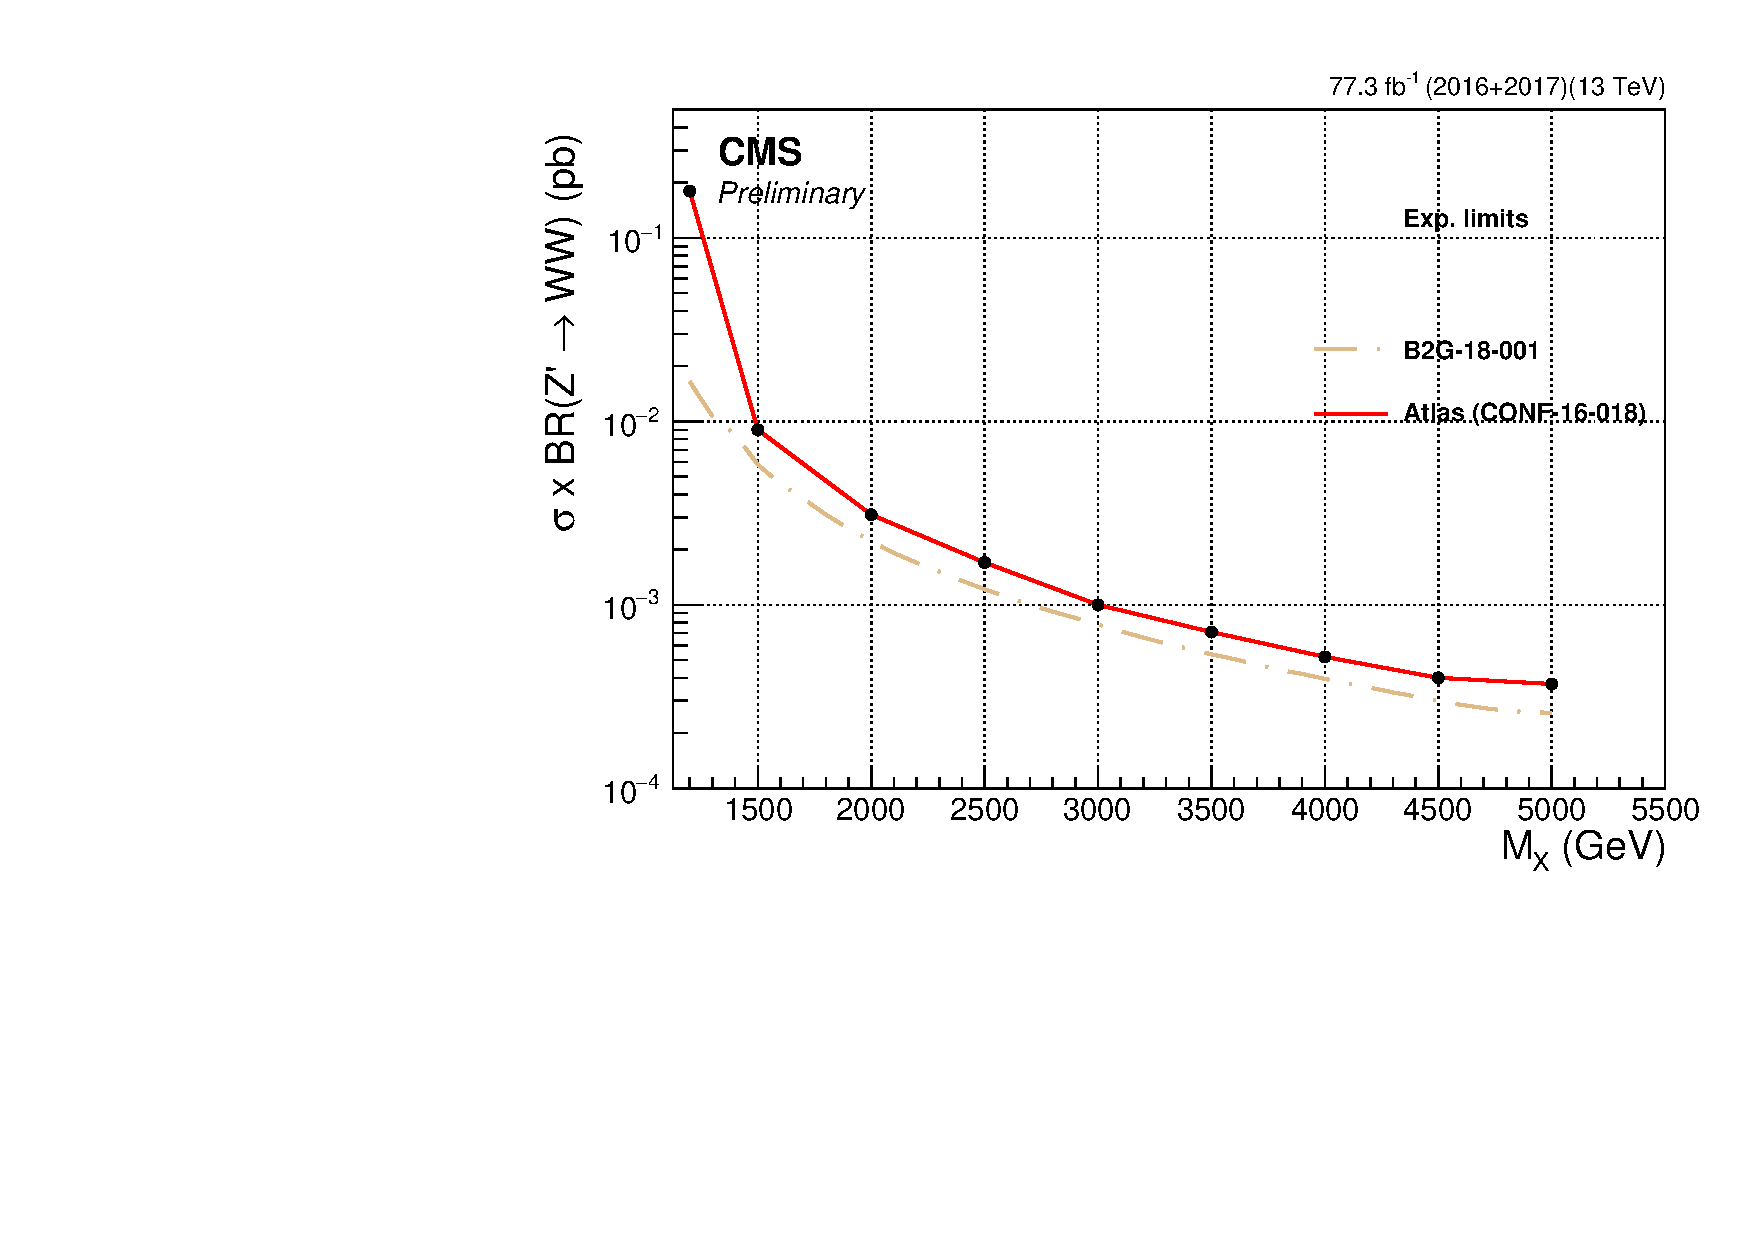
\includegraphics[width=0.69\columnwidth]{figures/compareLimits_Zprime_3D.pdf}
%\caption{Comparison of the expected limits for the search presented here to those obtained by the ATLAS collaboration in a similar search for a VV resonance decaying to hadrons~\cite{ATLAS-CONF-2018-016}.}
%\label{Fig8}
%\end{figure}
\section{Encoding jet substructure in a deep neural network}
\label{sec:DNN}
In an effort to go beyond current techniques to the next level, I have also developed a novel vector-boson tagger that uses all of the Lorentz vectors of the particles in the jet, and assembles the information using a deep neural network (DNN) in order to distinguish W and Z jets from quark and gluon jets~\cite{lola}. This algorithm yields twice the signal efficiency for a given mis-tagging rate with respect to current methods, and could significantly improve the sensitivity of future searches. Due to its special architecture, intended to encode jet substructure algorithms, it could also  be trained as a signal-independent tagger (separating quark/gluon jets from "any" potential signal jet). Together with the multi-dimensional framework, this could be used to design a truly model-independent search.

\section{SUMMARY}
As a Ph.D. student I have become a key contributor to the study of jet algorithms in the high-energy domain and provided essential studies for the improvement of jet tagging algorithms used in CMS. My work has allowed for the publication of dozens CMS analyses and has driven the field forward with original contributions. I have introduced a novel multi-dimensional search framework that, in addition to improving the search sensitivity by up to 35\%, allows us to easily incorporate alternate signal hypotheses, a key ingredient for future searches as no deviation has remained in the present data in searches for new resonances decaying into vector bosons. We are starting an era at LHC where improvements from adding more data are not where large sensitivity gains can be made anymore, but where real improvements in physics reach is obtained through improved methods. This new fit method, together with my work on improving vector-boson tagging, therefore makes this thesis highly relevant and important for future searches. My achievements include: the first demonstration of a Higgs(bb) tagging algorithm in CMS, bringing a highly anticipated result to publication as one of the first 13 TeV analyses, developing a new boson-tagging algorithm that is now default in CMS, providing kinematic-dependent corrections for vector-boson tagging between simulation and data, developing a brand new signal extraction method with a significantly improved sensitivity with respect to current methods, and demonstrating the first measurement of the SM V(qq)+jets background in diboson searches. I have also originated a deep neural network W/Z tagging algorithm, achieving a 50\% higher signal efficiency at a given mistag rate compared to current methods. In addition to my own work, I have had the pleasure and responsibility of supervising a CERN Summer Student on developing a tool to discriminate between transversally and longitudinally polarized vector bosons, and a bachelor student in the development of a b-tagging algorithm based only on number of hits in the pixel detector (see CV). Finally, I have been responsible for all pixel gain calibrations in 2017.


\bibliographystyle{auto_generated}
{\footnotesize
\bibliography{Bibliography.bib}}
\end{document}
